%% LyX 2.3.7 created this file.  For more info, see http://www.lyx.org/.
%% Do not edit unless you really know what you are doing.
\documentclass[journal,article,submit,pdftex,moreauthors]{Definitions/mdpi}
\usepackage[utf8]{inputenc}
\usepackage{float}
\usepackage{url}
\usepackage{graphicx}

\makeatletter

%%%%%%%%%%%%%%%%%%%%%%%%%%%%%% LyX specific LaTeX commands.

\Title{Neural DE: an evolutionary method based on Differential Evolution
suitable for neural network training}

\TitleCitation{Neural DE: an evolutionary method based on Differential Evolution
suitable for neural network training}

\Author{Ioannis G. Tsoulos$^{1,*}$, Vasileios Charilogis$^{2}$}

\AuthorNames{Ioannis G. Tsoulos; Vasileios Charilogis}

\AuthorCitation{Tsoulos, I.G.; Charilogis V.}


\address{$^{1}$\quad{}Department of Informatics and Telecommunications,
University of Ioannina, Greece;itsoulos@uoi.gr\\
$^{2}\quad$Department of Informatics and Telecommunications, University
of Ioannina, Greece; v.charilog@uoi.gr}


\corres{Correspondence: itsoulos@uoi.gr; }


\abstract{Artificial neural networks have proven to be an important machine
learning model that has been widely used in recent decades in a number
of difficult problems of classification or data fitting from real
- world areas. Due to their importance, a number of techniques have
been developed that efficiently identify the parameter vector for
these models. These techniques usually come from the field of optimization
and, by minimizing the training error of artificial neural networks,
estimate the vector of their parameters. However, many times these
techniques either get trapped in local minima of the training error
or lead to overfitting the artificial neural network, resulting in
poor performance when applied to data that was not present during
the training process. This paper presents an innovative training technique
for artificial neural networks based on the Differential Evolution
optimization method. This new technique creates an initial population
of artificial neural networks that evolve and periodically applies
a local optimization technique in order to accelerate the training
of these networks. The application of the local minimization technique
is done in such a way as to avoid the phenomenon of overfitting. This
new method was successfully applied to a series of classification
and data fitting problems and a comparative study was made with other
training techniques from the relevant literature.}


\keyword{Neural networks; Evolutionary methods; Differential Evolution; Machine
learning}

\DeclareTextSymbolDefault{\textquotedbl}{T1}
%% Because html converters don't know tabularnewline
\providecommand{\tabularnewline}{\\}

%%%%%%%%%%%%%%%%%%%%%%%%%%%%%% User specified LaTeX commands.
%  LaTeX support: latex@mdpi.com 
%  For support, please attach all files needed for compiling as well as the log file, and specify your operating system, LaTeX version, and LaTeX editor.

%=================================================================


% For posting an early version of this manuscript as a preprint, you may use "preprints" as the journal and change "submit" to "accept". The document class line would be, e.g., \documentclass[preprints,article,accept,moreauthors,pdftex]{mdpi}. This is especially recommended for submission to arXiv, where line numbers should be removed before posting. For preprints.org, the editorial staff will make this change immediately prior to posting.

%--------------------
% Class Options:
%--------------------
%----------
% journal
%----------
% Choose between the following MDPI journals:
% acoustics, actuators, addictions, admsci, adolescents, aerospace, agriculture, agriengineering, agronomy, ai, algorithms, allergies, alloys, analytica, animals, antibiotics, antibodies, antioxidants, applbiosci, appliedchem, appliedmath, applmech, applmicrobiol, applnano, applsci, aquacj, architecture, arts, asc, asi, astronomy, atmosphere, atoms, audiolres, automation, axioms, bacteria, batteries, bdcc, behavsci, beverages, biochem, bioengineering, biologics, biology, biomass, biomechanics, biomed, biomedicines, biomedinformatics, biomimetics, biomolecules, biophysica, biosensors, biotech, birds, bloods, blsf, brainsci, breath, buildings, businesses, cancers, carbon, cardiogenetics, catalysts, cells, ceramics, challenges, chemengineering, chemistry, chemosensors, chemproc, children, chips, cimb, civileng, cleantechnol, climate, clinpract, clockssleep, cmd, coasts, coatings, colloids, colorants, commodities, compounds, computation, computers, condensedmatter, conservation, constrmater, cosmetics, covid, crops, cryptography, crystals, csmf, ctn, curroncol, currophthalmol, cyber, dairy, data, dentistry, dermato, dermatopathology, designs, diabetology, diagnostics, dietetics, digital, disabilities, diseases, diversity, dna, drones, dynamics, earth, ebj, ecologies, econometrics, economies, education, ejihpe, electricity, electrochem, electronicmat, electronics, encyclopedia, endocrines, energies, eng, engproc, ent, entomology, entropy, environments, environsciproc, epidemiologia, epigenomes, est, fermentation, fibers, fintech, fire, fishes, fluids, foods, forecasting, forensicsci, forests, foundations, fractalfract, fuels, futureinternet, futureparasites, futurepharmacol, futurephys, futuretransp, galaxies, games, gases, gastroent, gastrointestdisord, gels, genealogy, genes, geographies, geohazards, geomatics, geosciences, geotechnics, geriatrics, hazardousmatters, healthcare, hearts, hemato, heritage, highthroughput, histories, horticulturae, humanities, humans, hydrobiology, hydrogen, hydrology, hygiene, idr, ijerph, ijfs, ijgi, ijms, ijns, ijtm, ijtpp, immuno, informatics, information, infrastructures, inorganics, insects, instruments, inventions, iot, j, jal, jcdd, jcm, jcp, jcs, jdb, jeta, jfb, jfmk, jimaging, jintelligence, jlpea, jmmp, jmp, jmse, jne, jnt, jof, joitmc, jor, journalmedia, jox, jpm, jrfm, jsan, jtaer, jzbg, kidney, kidneydial, knowledge, land, languages, laws, life, liquids, literature, livers, logics, logistics, lubricants, lymphatics, machines, macromol, magnetism, magnetochemistry, make, marinedrugs, materials, materproc, mathematics, mca, measurements, medicina, medicines, medsci, membranes, merits, metabolites, metals, meteorology, methane, metrology, micro, microarrays, microbiolres, micromachines, microorganisms, microplastics, minerals, mining, modelling, molbank, molecules, mps, msf, mti, muscles, nanoenergyadv, nanomanufacturing, nanomaterials, ncrna, network, neuroglia, neurolint, neurosci, nitrogen, notspecified, nri, nursrep, nutraceuticals, nutrients, obesities, oceans, ohbm, onco, oncopathology, optics, oral, organics, organoids, osteology, oxygen, parasites, parasitologia, particles, pathogens, pathophysiology, pediatrrep, pharmaceuticals, pharmaceutics, pharmacoepidemiology, pharmacy, philosophies, photochem, photonics, phycology, physchem, physics, physiologia, plants, plasma, pollutants, polymers, polysaccharides, poultry, powders, preprints, proceedings, processes, prosthesis, proteomes, psf, psych, psychiatryint, psychoactives, publications, quantumrep, quaternary, qubs, radiation, reactions, recycling, regeneration, religions, remotesensing, reports, reprodmed, resources, rheumato, risks, robotics, ruminants, safety, sci, scipharm, seeds, sensors, separations, sexes, signals, sinusitis, skins, smartcities, sna, societies, socsci, software, soilsystems, solar, solids, sports, standards, stats, stresses, surfaces, surgeries, suschem, sustainability, symmetry, synbio, systems, taxonomy, technologies, telecom, test, textiles, thalassrep, thermo, tomography, tourismhosp, toxics, toxins, transplantology, transportation, traumacare, traumas, tropicalmed, universe, urbansci, uro, vaccines, vehicles, venereology, vetsci, vibration, viruses, vision, waste, water, wem, wevj, wind, women, world, youth, zoonoticdis 

%---------
% article
%---------
% The default type of manuscript is "article", but can be replaced by: 
% abstract, addendum, article, book, bookreview, briefreport, casereport, comment, commentary, communication, conferenceproceedings, correction, conferencereport, entry, expressionofconcern, extendedabstract, datadescriptor, editorial, essay, erratum, hypothesis, interestingimage, obituary, opinion, projectreport, reply, retraction, review, perspective, protocol, shortnote, studyprotocol, systematicreview, supfile, technicalnote, viewpoint, guidelines, registeredreport, tutorial
% supfile = supplementary materials

%----------
% submit
%----------
% The class option "submit" will be changed to "accept" by the Editorial Office when the paper is accepted. This will only make changes to the frontpage (e.g., the logo of the journal will get visible), the headings, and the copyright information. Also, line numbering will be removed. Journal info and pagination for accepted papers will also be assigned by the Editorial Office.

%------------------
% moreauthors
%------------------
% If there is only one author the class option oneauthor should be used. Otherwise use the class option moreauthors.

%---------
% pdftex
%---------
% The option pdftex is for use with pdfLaTeX. If eps figures are used, remove the option pdftex and use LaTeX and dvi2pdf.

%=================================================================
% MDPI internal commands
\firstpage{1} 
 
\setcounter{page}{\@firstpage} 

\pubvolume{1}
\issuenum{1}
\articlenumber{0}
\pubyear{2022}
\copyrightyear{2022}
%\externaleditor{Academic Editor: Firstname Lastname} % For journal Automation, please change Academic Editor to "Communicated by"
\datereceived{} 
\dateaccepted{} 
\datepublished{} 
%\datecorrected{} % Corrected papers include a "Corrected: XXX" date in the original paper.
%\dateretracted{} % Corrected papers include a "Retracted: XXX" date in the original paper.
\hreflink{https://doi.org/} % If needed use \linebreak
%\doinum{}
%------------------------------------------------------------------
% The following line should be uncommented if the LaTeX file is uploaded to arXiv.org
%\pdfoutput=1

%=================================================================
% Add packages and commands here. The following packages are loaded in our class file: fontenc, inputenc, calc, indentfirst, fancyhdr, graphicx, epstopdf, lastpage, ifthen, lineno, float, amsmath, setspace, enumitem, mathpazo, booktabs, titlesec, etoolbox, tabto, xcolor, soul, multirow, microtype, tikz, totcount, changepage, attrib, upgreek, cleveref, amsthm, hyphenat, natbib, hyperref, footmisc, url, geometry, newfloat, caption

%=================================================================
%% Please use the following mathematics environments: Theorem, Lemma, Corollary, Proposition, Characterization, Property, Problem, Example, ExamplesandDefinitions, Hypothesis, Remark, Definition, Notation, Assumption
%% For proofs, please use the proof environment (the amsthm package is loaded by the MDPI class).

%=================================================================
% The fields PACS, MSC, and JEL may be left empty or commented out if not applicable
%\PACS{J0101}
%\MSC{}
%\JEL{}

%%%%%%%%%%%%%%%%%%%%%%%%%%%%%%%%%%%%%%%%%%
% Only for the journal Diversity
%\LSID{\url{http://}}

%%%%%%%%%%%%%%%%%%%%%%%%%%%%%%%%%%%%%%%%%%
% Only for the journal Applied Sciences:
%\featuredapplication{Authors are encouraged to provide a concise description of the specific application or a potential application of the work. This section is not mandatory.}
%%%%%%%%%%%%%%%%%%%%%%%%%%%%%%%%%%%%%%%%%%

%%%%%%%%%%%%%%%%%%%%%%%%%%%%%%%%%%%%%%%%%%
% Only for the journal Data:
%\dataset{DOI number or link to the deposited data set in cases where the data set is published or set to be published separately. If the data set is submitted and will be published as a supplement to this paper in the journal Data, this field will be filled by the editors of the journal. In this case, please make sure to submit the data set as a supplement when entering your manuscript into our manuscript editorial system.}

%\datasetlicense{license under which the data set is made available (CC0, CC-BY, CC-BY-SA, CC-BY-NC, etc.)}

%%%%%%%%%%%%%%%%%%%%%%%%%%%%%%%%%%%%%%%%%%
% Only for the journal Toxins
%\keycontribution{The breakthroughs or highlights of the manuscript. Authors can write one or two sentences to describe the most important part of the paper.}

%%%%%%%%%%%%%%%%%%%%%%%%%%%%%%%%%%%%%%%%%%
% Only for the journal Encyclopedia
%\encyclopediadef{Instead of the abstract}
%\entrylink{The Link to this entry published on the encyclopedia platform.}
%%%%%%%%%%%%%%%%%%%%%%%%%%%%%%%%%%%%%%%%%%

\makeatother

\begin{document}
\maketitle

\section{Introduction}

An artificial neural network \citep{nn1,nn2} is defined commonly
as\textbf{ }a function $N(\overrightarrow{x},\overrightarrow{w})$,
where the vector \textbf{$\overrightarrow{x}$ }stands for the input
pattern and the vector $\overrightarrow{w}$ (weight vector) represents
the vector of parameters for this particular network. This function
is used in classification and regression problems and the training
procedure refers to the adaptation of $\overrightarrow{w}$ by minimizing
the so-called training error defined as:
\begin{equation}
E\left(N\left(\overrightarrow{x},\overrightarrow{w}\right)\right)=\sum_{i=1}^{M}\left(N\left(\overrightarrow{x}_{i},\overrightarrow{w}\right)-y_{i}\right)^{2}\label{eq:eq1}
\end{equation}
Where the set $\left(\overrightarrow{x_{i}},y_{i}\right),\ i=1,...,M$\textbf{
}stands for the train set for the training process. The values $y_{i}$
denote the expected outputs for the $\overrightarrow{x_{i}}$ patterns.
These model have been applied successfully on a variety of cases from
real world problems, such as problems found in physics\textbf{ }\citep{nnphysics1,nnphysics2,nnphysics3},
problems related to the solution of differential equations \citep{nnde1},\textbf{
}problems related to solar radiation\citep{nn_solar},\textbf{ }agriculture
problems \citep{nnagr2},\textbf{ }problems appeared in chemistry
\citep{nnchem1,nnchem3},\textbf{ }economics problems \citep{nnecon1,nnecon2},
medicine problems \citep{nnmed1,nnmed2} etc.

Due to the widespread use of artificial neural networks, a significant
range of methods has been developed that identify the optimal parameter
vector by minimizing equation \ref{eq:eq1}. This set of methods included
the Back Propagation method\textbf{ }\citep{bpnn1,bpnn2}\textbf{,}
the RPROP method \citep{rpropnn-1}, the Adam optimizer\citep{Adam}
etc. Also, more recent approaches have been used to train artificial
neural networks such as the Simulated Annealing method \citep{nn_ann1},
modified version of the Genetic Algorithm \citep{geneticnn}, the
Particle Swarm Optimization (PSO) method \citep{psonn}, the Ant Colony
Optimization technique \citep{weight_aco} etc. Moreover, Sexton et
al. proposed the incorporation of the tabu search algorithm for neural
network training \citep{tabunn} and Zhang et al. suggested a hybrid
algorithm \citep{nn_hybrid} that utilizes the PSO method and the
Back Propagation method for efficient neural network training. Also,
Karaboga suggested the application of the Artificial Bee Colony (ABC)
algorithm to train artificial neural networks \citep{weight_abc}.
Recently, Zhao et al proposed a new Cascaded Forward Algorithm to
train artificial neural networks \citep{nn_cascade}. 

However, in many cases, although the above techniques can significantly
reduce the error of equation \ref{eq:eq1}, they lead the artificial
neural network to overfitting, that is, the network exhibits significantly
reduced performance on data that was not present during training.
This problem has been studied extensively in the relevant literature
and a number of methods have been proposed to address it, such as
weight sharing \citep{nnsharing1,nnsharing2}, pruning \citep{nnprunning1,nnprunning2},\textbf{
}early stopping \citep{nnearly1,nnearly2}, weight decaying \citep{nndecay1,nndecay2}
etc.

This paper proposed a new evolutionary optimization technique based
on Differential Evolution \citep{de_review} to efficiently train
artificial neural networks. The\textbf{ }Differential Evolution (DE)
method was initially proposed by Storn and Price \citep{de1,de2}
and it has been applied successfully on a variety of optimization
problems, such as community detection \citep{de_symmetry1}, structure
prediction \citep{de_symmetry3}, motor fault diagnosis \citep{de_symmetry6},
clustering techniques \citep{de_symmetry7} etc. The method also has
been used in machine learning applications, such as\textbf{ }as classification
methods \citep{key-16,de_problem2}, feature selection techniques
\citep{de_problem3,de_problem4}, deep learning \citep{de_deep1,de_deep2},
etc. In the current work a series of modifications are incorporated
in the DE method in order to efficient train artificial neural networks.
Among these modifications one finds the periodic and controlled application
of a local optimization method to randomly selected neural networks
from the population of the DE method. The application of the local
technique is done by ensuring that the parameters of the neural network
remain within a specific value range, thus avoiding, to the extent
possible, any overfitting that could occur. Furthermore, in the modifications
there is a termination rule that, on the one hand, is based on stochastic
observations regarding the evolution of the population of the DE method
and, on the other hand, uses the special characteristics of the error
function of the artificial neural network. 

The rest of this article is organized as follows: in section \ref{sec:The-proposed-method}
the proposed algorithm is fully outlined, in section \ref{sec:Experiments}
the datasets used in the experiments are listed accompanied by a series
of experiments regarding various aspects of the proposed method and
finally some conclusions are presented in section \ref{sec:Conclusions}.

\section{The proposed method\label{sec:The-proposed-method}}

The Differential Evolution method involves a series of candidate solutions
called agents. These agents evolve through a series of iterations
aiming to obtain the global minimum of the corresponding objective
function. In the present method, each agent also constitutes a vector
of parameters of an artificial neural network and the objective function
to be minimized is the error function presented previously. The neural
networks used in the current work are expressed through the equation:
\begin{equation}
N\left(\overrightarrow{x},\overrightarrow{w}\right)=\sum_{i=1}^{H}w_{(d+2)i-(d+1)}\sigma\left(\sum_{j=1}^{d}x_{j}w_{(d+2)i-(d+1)+j}+w_{(d+2)i}\right)\label{eq:nn}
\end{equation}
that was initially suggested in \citep{nnc}. The constant $H$ denotes
the number of processing units for the neural network and the constant
$d$ stands for the number of elements in the input pattern $\overrightarrow{x}$.
Hence, the number of elements in the parameter vector $\overrightarrow{w}$
are calculated as $n=\left(d+2\right)H$. The main steps of the proposed
method are as follows:
\begin{enumerate}
\item \textbf{Initialization Step}.
\begin{enumerate}
\item \textbf{Set} as NP the number of agents.
\item \textbf{Create} randomly the NP agents $g_{i},\ i=1,\ldots,\mbox{NP}$
\item \textbf{Compute} the fitness value $f_{i}$ of each agent $g_{i}$
using the objective function as $f_{i}=f\left(g_{i}\right)$.
\item \textbf{Set} as $p_{l}$ the local search rate.
\item \textbf{Set} as $a\ge1$ the weight parameter for the method.
\item \textbf{Set} as $N_{g}$ the maximum number of iterations allowed.
\item \textbf{Set} as $N_{I}$ the number of iterations used in the stopping
rule.
\item \textbf{Set} the parameter CR, which represents the crossover probability
with $\mbox{CR\ensuremath{\le1}}.$
\item \textbf{Set} $k=0$, the iteration counter.
\end{enumerate}
\item \textbf{Main Step}.\label{enu:Main-Step.}
\begin{enumerate}
\item \textbf{For $i=1,\ldots,$}NP\textbf{ do}
\begin{enumerate}
\item \textbf{Obtain} the agent $g_{i}$
\item \textbf{Select} randomly three distinct agents $g_{a},g_{b},g_{c}$. 
\item \textbf{Draw} a random integer $R\in[1,n]$.
\item \textbf{Create} a trial point $x_{t}$.
\item \textbf{For} $j=1,\ldots.n$ \textbf{do}
\begin{enumerate}
\item \textbf{Draw} a random number $r\in[0,1]$.
\item \textbf{If} $r\le\mbox{CR}$ \textbf{or} $i=R$ \textbf{then} $x_{t,j}=g_{a,j}+F\times\left(g_{b,j}-g_{c,j}\right)$
\textbf{else} $x_{t,j}=g_{i,j}$. The value $F$ represents the differential
weight of the DE method and it is calculated as 
\begin{equation}
F=-0.5+2r
\end{equation}
with $r$ a random number number in $[0,1]$. This calculation was
introduced in the paper of Charilogis et al \citep{de_char}.
\end{enumerate}
\item \textbf{End For}
\item \textbf{Set} $f_{t}=f\left(x_{t}\right)$
\item \textbf{If} $f_{t}\le f_{i}$ then $g_{i}=x_{t}$.
\item \textbf{Draw} a random number $r\in[0,1]$.
\item \textbf{If} $r\le p_{l}$ \textbf{then}
\begin{enumerate}
\item \textbf{Create} the vectors $\overrightarrow{L},\overrightarrow{R}$
with the properties
\[
\begin{array}{ccc}
L_{i} & = & -a\left|g_{i}\right|\\
R_{i} & = & a\left|g_{i}\right|
\end{array},\ i=1,\ldots,n
\]
.
\item \textbf{Minimize} the error function 
\begin{equation}
E\left(N\left(\overrightarrow{x},\overrightarrow{g_{i}}\right)\right)=\sum_{j=1}^{M}\left(N\left(\overrightarrow{x}_{j},\overrightarrow{g_{i}}\right)-y_{j}\right)^{2}\label{eq:eq1-1}
\end{equation}
 inside the bounds $\overrightarrow{L},\overrightarrow{R}$ using
some local optimization method. In the current work the BFGS variant
of Powell \citep{powell} was selected as the local optimization method.
\item \textbf{Set} $f_{i}=E\left(N\left(\overrightarrow{x},\overrightarrow{g_{i}}\right)\right)$.
\end{enumerate}
\item \textbf{End if}
\end{enumerate}
\item \textbf{End For}
\end{enumerate}
\item \textbf{Termination check Step}.
\begin{enumerate}
\item \textbf{Set} $k=k+1$.
\item \textbf{If} $k\ge N_{g}$ \textbf{then} goto step \ref{enu:Testing-step.}.
\item \textbf{Check} the termination rule specified in the work of Charilogis
et al \citep{de_char}. In this work the value 
\begin{equation}
\delta^{(k)}=\left|\sum_{i=1}^{\mbox{NP}}\left|f_{i}^{(k)}\right|-\sum_{i=1}^{\mbox{NP}}\left|f_{i}^{(k-1)}\right|\right|
\end{equation}
is calculated, where the value $f_{i}^{(k)}$ represents the fitness
value of agent $i$ at iteration $k$. If $\delta^{(k)}\le\epsilon$
for a number of $N_{I}$ iterations, then goto step \ref{enu:Testing-step.}.
\item \textbf{Obtain} the agent $g^{*}$ with the lowest fitness value $f^{*}$.
\item \textbf{If} $f^{*}\le e$ then goto step \ref{enu:Testing-step.}.
\item \textbf{Goto} step \ref{enu:Main-Step.}.
\end{enumerate}
\item \textbf{Testing step}.\label{enu:Testing-step.}
\begin{enumerate}
\item \textbf{Obtain} the agent $g^{*}$ with the lowest fitness value $f^{*}$.
\item \textbf{Apply} the neural network $N\left(\overrightarrow{x},\overrightarrow{g^{*}}\right)$
and report the associated test error.
\end{enumerate}
%
\end{enumerate}
The main steps of the proposed method are also outlined graphically
in Figure \ref{fig:flow_de}.

\begin{figure}[H]
\begin{centering}
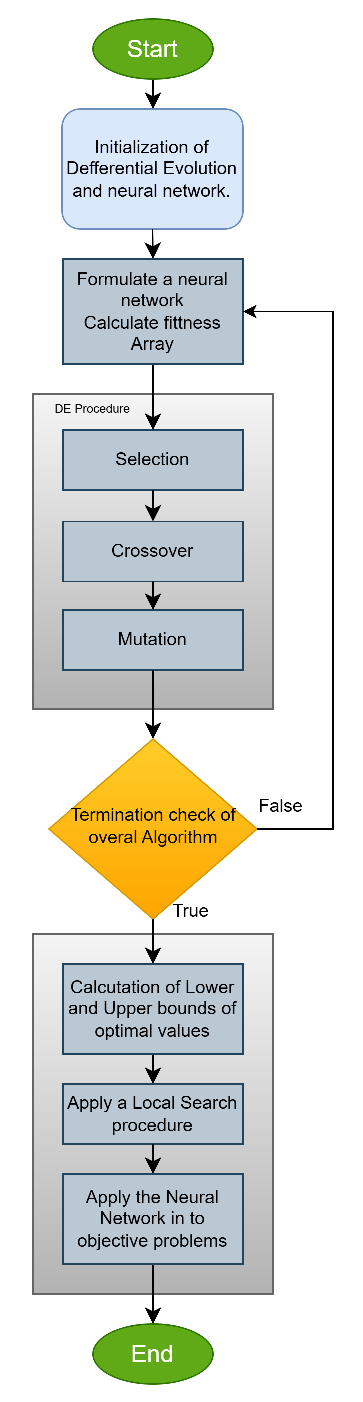
\includegraphics[scale=0.5]{neural_de.eps}
\par\end{centering}
\caption{The flowchart of the proposed method.\label{fig:flow_de}}

\end{figure}


\section{Experiments \label{sec:Experiments}}

A series of experiments were carried out to determine the effectiveness
of the proposed technique and its ability to achieve low generalization
errors in classification and data fitting problems. In addition, a
series of experiments were performed to determine the stability of
the method when critical parameters take different values. In order
to perform the experiments a series of classification and regression
datasets from the relevant literature was obtained. These datasets
can be found in the following websites:
\begin{enumerate}
\item The UCI website, \url{https://archive.ics.uci.edu/}(accessed on 9
January 2025)\citep{uci}
\item The Keel website, \url{https://sci2s.ugr.es/keel/datasets.php}(accessed
on 9 January 2025)\citep{Keel}.
\item The Statlib URL \url{https://lib.stat.cmu.edu/datasets/index}(accessed
on 9 January 2025). 
\end{enumerate}

\subsection{Experimental datasets }

The following series of classification datasets was used:
\begin{enumerate}
\item \textbf{Alcohol}, which is related to some experiments regarding alcohol
consumption \citep{alcohol}. 
\item \textbf{Australian}, which is related to bank transactions \citep{australian}.
\item \textbf{Bands,} regarding printing problems \citep{bands}.
\item \textbf{Balance} dataset \citep{balance}, which is related to psychological
experiments.
\item \textbf{Cleveland}, a medical dataset which was thoroughly studied
in the past in a series of research papers \citep{cleveland1,cleveland2}. 
\item \textbf{Circular} dataset, which created artificially. 
\item \textbf{Dermatology}, a medical dataset related to dermatology problems
\citep{dermatology}.
\item \textbf{Ecoli}, which is related to protein issues \citep{ecoli}.
\item \textbf{Haberman}, a medical dataset used for breast cancer detection.
\item \textbf{Hayes-roth} dataset \citep{hayes-roth}.
\item \textbf{Heart}, a dataset related to heart diseases \citep{heart}.
\item \textbf{HeartAttack}, a dataset related to heart diseases
\item \textbf{Hepatitis}, a medical dataset regarding hepatitis. 
\item \textbf{Housevotes}, that was used in the Congressional voting in
USA \citep{housevotes}.
\item \textbf{Ionosphere}, a dataset related to measurements from the ionosphere
\citep{ion1,ion2}.
\item \textbf{Liverdisorder}, which is a medical dataset studied in a series
of papers\citep{liver,liver1}.
\item \textbf{Lymography} \citep{lymography}.
\item \textbf{Magic}, this dataset contains measurements from physics simulations
\citep{magic}.
\item \textbf{Mammographic}, a medical dataset related to breast cancer
\citep{mammographic}.
\item \textbf{Page Blocks }dataset \citep{pageblocks}, related to the page
layout of documents.
\item \textbf{Parkinsons}, a medical dataset for the detection of Parkinson's
disease \citep{parkinsons1,parkinsons2}.
\item \textbf{Pima}, a medical dataset related to the presence of diabetes\citep{pima}.
\item \textbf{Phoneme}, a dataset regarding sounds.
\item \textbf{Popfailures}, a dataset related to measurements from climate
experiments \citep{popfailures}.
\item \textbf{Regions2}, a medical dataset used for the detection of issues
in the liver \citep{regions2}.
\item \textbf{Ring}, a dataset related to a series of multivariate normal
distributions. 
\item \textbf{Saheart}, used for the detection of heart diseases.\citep{saheart}.
\item \textbf{Segment} dataset \citep{segment}.
\item \textbf{Statheart}, a medical dataset used for the detection of heart
diseases.
\item \textbf{Sonar} dataset \citep{sonar}.
\item \textbf{Spambase}, a dataset used to recognize spam emails. 
\item \textbf{Spiral}, which is an artificial dataset.
\item \textbf{Student}, a dataset concerning experiments in schools \citep{student}.
\item \textbf{Tae}, used to evaluate teaching performance.
\item \textbf{Transfusion}, which is a medical dataset \citep{transfusion}.
\item \textbf{Wdbc}, a medical dataset which is used to detect breast cancer
\citep{wdbc1,wdbc2}.
\item \textbf{Wine}, a dataset used to detect the quality of wines \citep{wine1,wine2}.
\item \textbf{EEG} dataset, which is a medical dataset about EEG recordings\citep{eeg1,eeg2}.
The following cases from this dataset were adopted here: Z\_F\_S,
ZO\_NF\_S and ZONF\_S.
\item \textbf{Zoo}, a dataset used for animal classification \citep{zoo}
.
\end{enumerate}
Additionally, the following series of regression datasets was adopted:
\begin{enumerate}
\item \textbf{Abalone}, a dataset related to the age of abalones \citep{abalone}.
\item \textbf{Airfoil}, a dataset provided by NASA \citep{airfoil}.
\item \textbf{Auto}, a dataset related to the fuel consumption of cars.
\item \textbf{BK}, a dataset which is related to basketball games. 
\item \textbf{BL}, a dataset related to electricity experiments.
\item \textbf{Baseball}, a dataset used to estimate the income of baseball
players.
\item \textbf{Concrete}, a civil engineering dataset \citep{concrete}.
\item \textbf{DEE}, used for the prediction of electricity prices.
\item \textbf{FA}, that contains measurements about body fat.
\item \textbf{Friedman}, an artificial dataset\citep{friedman}.
\item \textbf{FY, }this dataset used in experiments regarding the longevity
of fruit flies. 
\item \textbf{HO}, a dataset with 13 features obtained from the STATLIB
repository.
\item \textbf{Housing}, used to estimate the price of houses \citep{housing}.
\item \textbf{Laser}, used in a series of laser experiments.
\item \textbf{LW}, a dataset used to detect the weight of babes.
\item \textbf{Mortgage}, an dataset related to economic measurements.
\item \textbf{Plastic}, a dataset related to problems regarding pressure
on plastics.
\item \textbf{PY }dataset, (Pyrimidines problem). The task of this dataset
is the learning of Learning Quantitative Structure Activity Relationships
(QSARs)\citep{pydataset}.
\item \textbf{Quake}, a dataset used to measure earthquakes.
\item \textbf{SN}, a dataset related to trellising and pruning.
\item \textbf{Stock}, a dataset related to the prices of stocks.
\item \textbf{Treasury}, which is related to economics.
\end{enumerate}

\subsection{Experimental results}

The code used in the current work was implemented using the C++ programming
language and the Optimus optimization library, freely available from\textbf{
}\url{https://github.com/itsoulos/OPTIMUS} (accessed on 9 January
2025). Every experiment was repeated 30 times, using different seed
for the random number generator each time. For the validation of the
experiments the 10 - fold cross validation technique was incorporated.
The machine used in the experiments was an AMD Ryzen 5950X with 128GB
of ram, running Debian Linux as the operating system. The values for
the parameters of the proposed method are listed in Table\textbf{
}\ref{tab:settings}.\textbf{ }
\begin{table}[H]
\caption{The values for the parameters of the proposed method.\label{tab:settings}}

\centering{}%
\begin{tabular}{|c|c|c|}
\hline 
PARAMETER & MEANING & VALUE\tabularnewline
\hline 
\hline 
$N_{g}$ & Number of maximum allowed generations. & 200\tabularnewline
\hline 
NP & Number of agents & 500\tabularnewline
\hline 
CR & Crossover probability & 0.9\tabularnewline
\hline 
$N_{I}$ & Number of iterations for termination rule & 10\tabularnewline
\hline 
$p_{l}$ & Local search rate & 0.005\tabularnewline
\hline 
$a$ & Weight parameter & 2.0\tabularnewline
\hline 
$H$ & Number of processing nodes for neural network & 10\tabularnewline
\hline 
\end{tabular}
\end{table}
\textbf{ }

The table \ref{tab:experClass} depicts the experimental results for
the classification datasets and Table \ref{tab:experRegression} shows
the experimental results for the regression datasets.\textbf{ }The
used formula for the classification error is:
\begin{equation}
E_{C}\left(M(x)\right)=100\times\frac{\sum_{i=1}^{N}\left(\mbox{class}\left(M\left(x_{i}\right)\right)-y_{i}\right)}{N}
\end{equation}
where $M(x)$ denotes the used model and the set $T$ represents the
train dataset.\textbf{ }Likewise, the regression error is defined
as:
\begin{equation}
E_{R}\left(M(x)\right)=\frac{\sum_{i=1}^{N}\left(M\left(x_{i}\right)-y_{i}\right)^{2}}{N}
\end{equation}
In all experimental tables the following notation was adopted:
\begin{enumerate}
\item The column DATASET denotes the name of the used dataset.
\item The column ADAM represents the incorporation of the ADAM optimizer
for the training of a neural network with $H=10$ processing nodes.
\item The column BFGS stands for the usage of the BFGS optimization method
provided by Powell \citep{powell} for the training of a neural network
with~$H=10$ processing nodes.
\item The column GENETIC represents the usage of a genetic algorithm for
the training of a neural network with $H=10$ processing nodes. The
number of chromosomes in this genetic algorithm are equal with the
number of agents in the proposed method.
\item The column NEAT stands for the usage of the NEAT method (NeuroEvolution
of Augmenting Topologies ) \citep{neat} for the training of a neural
network. This method was implemented in \url{https://github.com/BiagioFesta/EvolutionNet}(accessed
on 9 January 2025). 
\item The column RBF represents the usage of a Radial Basis Function (RBF)
network \citep{rbf1,rbf2} with $H=10$ processing nodes.
\item The row AVERAGE stands for the average classification or regression
error for all datasets in the corresponding table.
\end{enumerate}
\begin{table}[H]
\caption{Experimental results for the classification datasets using the series
of optimization methods. The numbers in cells represent average classification
error measured on the corresponding test set.\label{tab:experClass}}

\centering{}%
\begin{tabular}{|c|c|c|c|c|c|c|}
\hline 
DATASET & ADAM & BFGS & GENETIC & NEAT & RBF & NEURALDE\tabularnewline
\hline 
\hline 
ALCOHOL & 57.78\% & 41.50\% & 39.57\% & 66.80\% & 49.32\% & 19.15\%\tabularnewline
\hline 
AUSTRALIAN & 35.65\% & 38.13\% & 32.21\% & 31.98\% & 34.89\% & 15.31\%\tabularnewline
\hline 
BALANCE & 12.27\% & 8.64\% & 8.97\% & 23.14\% & 33.53\% & 6.92\%\tabularnewline
\hline 
BANDS & 36.92\% & 36.67\% & 34.92\% & 34.30\% & 37.17\% & 35.00\%\tabularnewline
\hline 
CLEVELAND & 67.55\% & 77.55\% & 51.60\% & 53.44\% & 67.10\% & 45.07\%\tabularnewline
\hline 
CIRCULAR & 19.95\% & 6.08\% & 5.99\% & 35.18\% & 5.98\% & 4.23\%\tabularnewline
\hline 
DERMATOLOGY & 26.14\% & 52.92\% & 30.58\% & 32.43\% & 62.34\% & 10.38\%\tabularnewline
\hline 
ECOLI & 64.43\% & 69.52\% & 54.67\% & 43.44\% & 59.48\% & 45.22\%\tabularnewline
\hline 
HABERMAN & 29.00\% & 29.34\% & 28.66\% & 24.04\% & 25.10\% & 27.55\%\tabularnewline
\hline 
HAYES-ROTH & 59.70\% & 37.33\% & 56.18\% & 50.15\% & 64.36\% & 35.59\%\tabularnewline
\hline 
HEART & 38.53\% & 39.44\% & 28.34\% & 39.27\% & 31.20\% & 17.60\%\tabularnewline
\hline 
HEARTATTACK & 45.55\% & 46.67\% & 29.03\% & 32.34\% & 29.00\% & 19.70\%\tabularnewline
\hline 
HEPATITIS & 68.13\% & 72.47\% & 62.12\% & 67.04\% & 64.63\% & 57.46\%\tabularnewline
\hline 
HOUSEVOTES & 7.48\% & 7.13\% & 6.62\% & 10.89\% & 6.13\% & 7.48\%\tabularnewline
\hline 
IONOSPHERE & 16.64\% & 15.29\% & 15.14\% & 19.67\% & 16.22\% & 16.17\%\tabularnewline
\hline 
LIVERDISORDER & 41.53\% & 42.59\% & 31.11\% & 30.67\% & 30.84\% & 31.72\%\tabularnewline
\hline 
LYMOGRAPHY & 39.79\% & 35.43\% & 28.42\% & 33.70\% & 25.50\% & 28.86\%\tabularnewline
\hline 
MAGIC & 40.55\% & 17.30\% & 21.75\% & 24.85\% & 21.28\% & 11.73\%\tabularnewline
\hline 
MAMMOGRAPHIC & 46.25\% & 17.24\% & 19.88\% & 22.85\% & 21.38\% & 17.52\%\tabularnewline
\hline 
PARKINSONS & 24.06\% & 27.58\% & 18.05\% & 18.56\% & 17.41\% & 14.32\%\tabularnewline
\hline 
PAGE BLOCKS & 34.27\% & 8.49\% & 6.84\% & 10.22\% & 10.09\% & 6.04\%\tabularnewline
\hline 
PHONEME & 29.43\% & 15.58\% & 15.55\% & 22.34\% & 23.32\% & 15.50\%\tabularnewline
\hline 
PIMA & 34.85\% & 35.59\% & 32.19\% & 34.51\% & 25.78\% & 24.85\%\tabularnewline
\hline 
POPFAILURES & 5.18\% & 5.24\% & 5.94\% & 7.05\% & 7.04\% & 6.09\%\tabularnewline
\hline 
REGIONS2 & 29.85\% & 36.28\% & 29.39\% & 33.23\% & 38.29\% & 28.77\%\tabularnewline
\hline 
RING & 28.80\% & 29.44\% & 28.80\% & 30.85\% & 21.67\% & 22.90\%\tabularnewline
\hline 
SAHEART & 34.04\% & 37.48\% & 34.86\% & 34.51\% & 32.19\% & 29.63\%\tabularnewline
\hline 
SEGMENT & 49.75\% & 68.97\% & 57.72\% & 66.72\% & 59.68\% & 15.60\%\tabularnewline
\hline 
SONAR & 30.33\% & 25.85\% & 22.40\% & 34.10\% & 27.90\% & 19.80\%\tabularnewline
\hline 
SPAMBASE & 48.05\% & 18.16\% & 6.37\% & 35.77\% & 29.35\% & 4.95\%\tabularnewline
\hline 
SPIRAL & 47.67\% & 47.99\% & 48.66\% & 48.66\% & 44.87\% & 42.06\%\tabularnewline
\hline 
STATHEART & 44.04\% & 39.65\% & 27.25\% & 44.36\% & 31.36\% & 18.53\%\tabularnewline
\hline 
STUDENT & 5.13\% & 7.14\% & 5.61\% & 10.20\% & 5.49\% & 4.86\%\tabularnewline
\hline 
TAE & 60.20\% & 51.58\% & 49.84\% & 60.67\% & 60.02\% & 45.62\%\tabularnewline
\hline 
TRANSFUSION & 25.68\% & 25.84\% & 24.87\% & 24.87\% & 26.41\% & 23.59\%\tabularnewline
\hline 
WDBC & 35.35\% & 29.91\% & 8.56\% & 12.88\% & 7.27\% & 4.29\%\tabularnewline
\hline 
WINE & 29.40\% & 59.71\% & 19.20\% & 25.43\% & 31.41\% & 10.39\%\tabularnewline
\hline 
Z\_F\_S & 47.81\% & 39.37\% & 10.73\% & 38.41\% & 13.16\% & 6.81\%\tabularnewline
\hline 
ZO\_NF\_S & 47.43\% & 43.04\% & 21.54\% & 43.75\% & 9.02\% & 4.73\%\tabularnewline
\hline 
ZONF\_S & 11.99\% & 15.62\% & 4.36\% & 5.44\% & 4.03\% & 2.41\%\tabularnewline
\hline 
ZOO & 14.13\% & 10.70\% & 9.50\% & 20.27\% & 21.93\% & 6.63\%\tabularnewline
\hline 
\textbf{AVERAGE} & \textbf{35.88\%} & \textbf{33.43\%} & \textbf{26.19\%} & \textbf{32.66\%} & \textbf{30.08\%} & \textbf{19.78\%}\tabularnewline
\hline 
\end{tabular}
\end{table}
\begin{table}[H]
\caption{Experimental results for the provided regression datasets using the
series of methods. Numbers in cells represents average regression
error calculated on the corresponding test set.\label{tab:experRegression}}

\centering{}%
\begin{tabular}{|c|c|c|c|c|c|c|}
\hline 
DATASET & ADAM & BFGS & GENETIC & NEAT & RBF & NEURALDE\tabularnewline
\hline 
\hline 
ABALONE & 4.30 & 5.69 & 7.17 & 9.88 & 7.37 & 5.04\tabularnewline
\hline 
AIRFOIL & 0.005 & 0.003 & 0.003 & 0.067 & 0.27 & 0.0014\tabularnewline
\hline 
AUTO & 70.84 & 60.97 & 12.18 & 56.06 & 17.87 & 16.21\tabularnewline
\hline 
BK & 0.0252 & 0.28 & 0.027 & 0.15 & 0.02 & 0.019\tabularnewline
\hline 
BL & 0.622 & 2.55 & 5.74 & 0.05 & 0.013 & 0.016\tabularnewline
\hline 
BASEBALL & 77.90 & 119.63 & 103.60 & 100.39 & 93.02 & 60.56\tabularnewline
\hline 
CONCRETE & 0.078 & 0.066 & 0.0099 & 0.081 & 0.011 & 0.003\tabularnewline
\hline 
DEE & 0.63 & 2.36 & 1.013 & 1.51 & 0.17 & 0.35\tabularnewline
\hline 
FA & 0.048 & 0.426 & 0.025 & 0.19 & 0.015 & 0.083\tabularnewline
\hline 
FRIEDMAN & 22.90 & 1.263 & 1.249 & 19.35 & 7.23 & 1.22\tabularnewline
\hline 
HO & 0.035 & 0.62 & 2.78 & 0.17 & 0.03 & 0.017\tabularnewline
\hline 
HOUSING & 80.99 & 97.38 & 43.26 & 56.49 & 57.68 & 24.82\tabularnewline
\hline 
LASER & 0.03 & 0.015 & 0.59 & 0.084 & 0.03 & 0.0026\tabularnewline
\hline 
LW & 0.028 & 2.98 & 1.90 & 0.17 & 0.03 & 0.021\tabularnewline
\hline 
MORTGAGE & 9.24 & 8.23 & 2.41 & 14.11 & 1.45 & 0.54\tabularnewline
\hline 
PLASTIC & 11.71 & 20.32 & 2.791 & 20.77 & 8.62 & 3.27\tabularnewline
\hline 
PY & 0.321 & 0.578 & 0.56 & 0.075 & 0.012 & 0.11\tabularnewline
\hline 
QUAKE & 0.07 & 0.42 & 0.04 & 0.298 & 0.07 & 0.042\tabularnewline
\hline 
SN & 0.026 & 0.40 & 2.95 & 0.174 & 0.027 & 0.027\tabularnewline
\hline 
STOCK & 180.89 & 302.43 & 3.88 & 215.82 & 12.23 & 3.40\tabularnewline
\hline 
TREASURY & 11.16 & 9.91 & 2.93 & 15.52 & 2.02 & 1.021\tabularnewline
\hline 
\textbf{AVERAGE} & \textbf{22.47} & \textbf{30.31} & \textbf{9.29} & \textbf{24.35} & \textbf{9.91} & \textbf{5.56}\tabularnewline
\hline 
\end{tabular}
\end{table}

The analysis of Table \ref{tab:experClass} evaluates the error rates
of various machine learning models across multiple classification
datasets. Each row corresponds to a dataset, and each column represents
a specific model. The values indicate the error percentages, where
lower values signify better performance. The last row provides the
average error rate for each model, offering an overall performance
summary. Starting with the averages, the NEURALDE model exhibits the
best overall performance, achieving the lowest mean error rate of
19.78\%. It is followed by GENETIC with an average error rate of 26.19\%
and RBF at 30.08\%. The NEAT model has an average error rate of 32.66\%,
while BFGS and ADAM display the highest average error rates, 33.43\%
and 35.88\%, respectively. This makes NEURALDE the most efficient
model among those compared. On a dataset-specific level, NEURALDE
consistently delivers the lowest error rates in numerous cases. For
instance, in the ALCOHOL dataset, it achieves the best result with
an error rate of 19.15\%. Similarly, in the CIRCULAR dataset, NEURALDE
outperforms all other models with an error rate of 4.23\%, demonstrating
its effectiveness in handling complex data structures. In the MAGIC
and MAMMOGRAPHIC datasets, NEURALDE again proves superior, with error
rates of 11.73\% and 17.52\%, respectively. There are, however, a
few datasets where NEURALDE does not perform as dominantly. For example,
in the HOUSEVOTES dataset, it ties with other models at 7.48\%. In
the ZONF\_S dataset, it records its worst performance with an error
rate of 2.41\%, indicating that its efficiency can vary with certain
data characteristics. Other models, such as GENETIC, show strong performance
in isolated cases, such as in the SPIRAL dataset (48.66\%). However,
they generally fall short of NEURALDE’s consistent excellence. RBF
demonstrates strong stability, with notable results in the DERMATOLOGY
(62.34\%) and PHONEME (23.32\%) datasets. Meanwhile, ADAM and BFGS
tend to underperform, particularly in datasets like SPAMBASE, where
they record high error rates of 48.05\% and 18.16\%, respectively.
In conclusion, the NEURALDE model stands out as the most effective
model overall, achieving the lowest average error rate and excelling
in the majority of datasets. While other models, such as RBF and GENETIC,
perform well in specific scenarios, NEURALDE demonstrates superior
consistency and effectiveness across a wide range of datasets.

The Table \ref{tab:experRegression} presents the performance of various
machine learning models on regression problems, where the values represent
the error. Lower error values indicate better performance. Each row
corresponds to a specific dataset, while the last row shows the average
error for each model, providing an overall view of their effectiveness.Based
on the average error, NEURALDE demonstrates the best performance,
with the lowest overall error of 5.56. This result suggests that the
model consistently performs well across most datasets. Following NEURALDE
are GENETIC with an average error of 9.29 and RBF with an average
error of 9.91. ADAM, NEAT, and BFGS exhibit higher average errors,
at 22.47, 24.35, and 30.31 respectively, indicating lower performance
compared to the other models. Analyzing the results dataset by dataset,
NEURALDE records the smallest error in several cases. For instance,
in the AIRFOIL dataset, it achieves an error of 0.0014, outperforming
all other models. In the CONCRETE dataset, its error is only 0.003,
the lowest among all models. Similarly, in the LASER dataset, it achieves
an exceptionally low error of 0.0026. In the TREASURY dataset, NEURALDE
demonstrates superior performance with an error of 1.021, better than
all other models. GENETIC shows competitive performance in several
datasets. For example, in the HOUSING dataset, it achieves an error
of 43.26, which is better than ADAM and NEAT but not as strong as
NEURALDE. In the PLASTIC dataset, its error is 2.791, which is significantly
lower than most other models except NEURALDE.

RBF achieves low errors in some datasets, such as MORTGAGE, where
it records an error of 1.45, the second-best result after NEURALDE
(0.54). However, in other datasets like STOCK, where it has an error
of 12.23, RBF underperforms compared to GENETIC and NEURALDE. ADAM
and NEAT exhibit higher errors across many datasets. For example,
in the STOCK dataset, ADAM records the highest error at 180.89, followed
by NEAT at 215.82. Conversely, in the AIRFOIL dataset, ADAM achieves
a relatively low error of 0.005, though it still falls short of NEURALDE.
BFGS generally shows higher errors, such as in the BASEBALL dataset
(119.63), reflecting its limited performance. In summary, NEURALDE
stands out as the most effective regression model, with consistently
low errors and the lowest average error overall. GENETIC and RBF display
competitive performance in some datasets but lack the same consistency.
ADAM, NEAT, and BFGS exhibit significantly higher errors, indicating
their inferior performance compared to NEURALDE. 

An extensive analysis was conducted on the performance of different
machine learning models using various optimization methods, with pairwise
comparisons made through the Wilcoxon Test. The study was carried
out on a set of well-known datasets and focused on the NEURALDE model,
comparing it with other popular optimization methods such as ADAM,
BFGS, GENETIC, NEAT, and RBF. The Wilcoxon Test, a non-parametric
statistical method, is ideal for evaluating performance differences,
especially when the data does not follow a normal distribution Figure
\ref{fig:statClass}. The results revealed significant performance
differences between NEURALDE and other models. Specifically, the p-value
for the comparison between NEURALDE and ADAM was p=4.7e-08, a very
low value that indicates the differences between the two models are
statistically significant and unlikely to be due to chance. The p-value
for the comparison between NEURALDE and BFGS was even lower, at p=1e-18,
suggesting substantial performance differences, with NEURALDE outperforming
BFGS by a wide margin. Similarly, the comparison between NEURALDE
and GENETIC yielded p=2.9e-09, confirming that the two methods show
distinct performance, with NEURALDE being superior. The comparison
between NEURALDE and NEAT showed p=2.3e-10, while the comparison with
RBF resulted in p=1.3e-08. In both cases, the p-values were extremely
low, proving that the performance differences are statistically significant.
This analysis highlights NEURALDE as a standout model among the datasets
used, showing significant performance differences compared to the
other methods. The very low p-values in all comparisons demonstrate
that the observed differences are not due to random chance, but rather
reflect the true superiority or differentiation of NEURALDE. The methods
ADAM, BFGS, GENETIC, NEAT, and RBF are widely used and effective in
many cases, but this analysis suggests that NEURALDE excels in specific
problems or datasets. This statistical analysis provides valuable
insight into the selection of appropriate models and optimization
methods for machine learning tasks. Although the specific p-values
and results pertain to the datasets used in this study, the significance
of the findings underscores the importance of careful evaluation when
selecting models.

\begin{figure}[H]
\begin{centering}
\includegraphics[scale=0.5]{s1}
\par\end{centering}
\caption{Statistical comparison of the used machine learning models for the
classification datasets.\label{fig:statClass}}

\end{figure}

Furthermore, an analysis was conducted to compare various machine
learning models employing different optimization methods in terms
of regression error. The study was performed using a script in R,
employing the Wilcoxon Test for pairwise comparisons. This non-parametric
statistical test is suitable for data that do not follow a normal
distribution Figure \ref{fig:statRegression}. The experiments were
conducted on a series of well-known datasets, ensuring diversity across
problem domains. The results revealed significant differences in regression
error between the NEURALDE model and other optimization methods. Specifically,
the comparison between NEURALDE and ADAM yielded a p-value of 0.00051,
indicating a statistically significant difference in favor of NEURALDE.
Similarly, the comparison with BFGS showed an even smaller p-value
of 9.5e-07, highlighting the clear superiority of NEURALDE in this
context. The analysis of NEURALDE against GENETIC resulted in a p-value
of 0.0033, further supporting the significance of the observed difference.
Likewise, the comparison with NEAT gave a p-value of 2.9e-06, and
with RBF, the p-value was 0.0048, demonstrating statistically significant
differences in all cases. These findings indicate that NEURALDE consistently
outperforms the other optimization methods analyzed in terms of reducing
regression error. The exceptionally low p-values across all comparisons
suggest that these differences are unlikely to be due to random variation
and reflect a genuine advantage. While other methods such as ADAM,
BFGS, GENETIC, NEAT, and RBF are generally effective across various
tasks, the results show that NEURALDE exhibits superior performance
in minimizing regression error for the datasets analyzed. This analysis
provides valuable insights for selecting appropriate models and optimization
techniques in regression tasks. Although the results are specific
to the datasets used in the study, the statistical significance of
the findings highlights the importance of careful evaluation when
choosing a model. 

\begin{figure}[H]
\begin{centering}
\includegraphics[scale=0.5]{s2}
\par\end{centering}
\caption{Statistical comparison between the machine learning models for the
regression datasets.\label{fig:statRegression}}

\end{figure}


\subsubsection{Experiments with the differential weight }

Another series of experiments was carried out in order to determine
the effect that the specific differential weight calculation mechanism
has on the accuracy of the proposed technique. For this reason the
following methods for the calculation of the differential weight (parameter
$F$) were used:
\begin{itemize}
\item The method denoted as MIGRANT in the experimental tables. In this
case the differential weight mechanism proposed in \citep{de_migrant}
was used.
\item The method denoted as ADAPTIVE in the experimental tables. This method
uses the differential weight calculation proposed in \citep{de_dynamic}.
\item The method represented as RANDOM in the experimental tables. This
method is the default method, suggested by Charilogis \citep{de_char}. 
\end{itemize}
The table \ref{tab:experFClass} provides the performance of three
differential weight computation methods (MIGRANT, ADAPTIVE, and RANDOM)
on the series of classification datasets. The analysis reveals that
the MIGRANT method achieves the smallest average error rate of 19.34\%,
indicating the best overall performance among the three methods. The
RANDOM method follows closely with an average error rate of 19.78\%,
while the ADAPTIVE method has the highest average error rate of 19.98\%,
suggesting it is the least effective on average. Examining individual
datasets, MIGRANT outperforms the other methods in several cases.
For example, in the HEART dataset, MIGRANT records an error rate of
19.01\%, better than ADAPTIVE (17.29\%) and RANDOM (17.60\%). Similarly,
in the MAGIC dataset, MIGRANT achieves a competitive error rate of
11.83\%, which is close to RANDOM (11.73\%) but higher than ADAPTIVE
(11.28\%). MIGRANT also has the lowest error in datasets such as ALCOHOL
(19.62\%), REGIONS2 (26.26\%), and SPAMBASE (5.87\%). ADAPTIVE demonstrates
strong performance in specific datasets, achieving the lowest error
rates in cases such as MAGIC (11.28\%) and HEART (17.29\%). However,
in many datasets, it performs worse than MIGRANT or RANDOM, such as
in SPAMBASE, where it records a lower error rate of 4.78\% but is
generally outperformed in other critical datasets. The RANDOM method
exhibits competitive performance in several datasets, achieving the
lowest error rates in examples like ZOO (6.63\%) and ZONF\_S (2.41\%).
However, its performance fluctuates more significantly, with higher
error rates in datasets such as HEARTATTACK (19.70\%) and REGIONS2
(28.77\%), where it is outperformed by MIGRANT and ADAPTIVE. Notable
observations include cases where the error rates are very close across
the methods, such as in datasets like CIRCULAR, where the differences
are minimal (MIGRANT at 4.28\%, ADAPTIVE at 4.34\%, and RANDOM at
4.23\%). In other cases, the differences are more pronounced, as in
SEGMENT, where MIGRANT achieves 9.71\%, significantly better than
ADAPTIVE (15.99\%) and RANDOM (15.60\%). Overall, MIGRANT demonstrates
the most consistent and robust performance across the datasets, with
the lowest average error and competitive results in many individual
datasets. RANDOM and ADAPTIVE have comparable average errors but show
more variability in their performance.

\begin{table}[H]
\caption{Experimental results for the classification datasets using a list
of proposed differential weight mechanisms found in the literature.
\label{tab:experFClass}}

\centering{}%
\begin{tabular}{|c|c|c|c|}
\hline 
DATASET & MIGRANT & ADAPTIVE & RANDOM\tabularnewline
\hline 
\hline 
ALCOHOL & 19.62\% & 18.44\% & 19.15\%\tabularnewline
\hline 
AUSTRALIAN & 14.77\% & 16.14\% & 15.31\%\tabularnewline
\hline 
BALANCE & 6.79\% & 6.94\% & 6.92\%\tabularnewline
\hline 
BANDS & 33.28\% & 35.42\% & 35.00\%\tabularnewline
\hline 
CLEVELAND & 45.74\% & 44.60\% & 45.07\%\tabularnewline
\hline 
CIRCULAR & 4.28\% & 4.34\% & 4.23\%\tabularnewline
\hline 
DERMATOLOGY & 11.41\% & 9.83\% & 10.38\%\tabularnewline
\hline 
ECOLI & 42.61\% & 47.51\% & 45.22\%\tabularnewline
\hline 
HABERMAN & 27.76\% & 28.35\% & 27.55\%\tabularnewline
\hline 
HAYES-ROTH & 35.92\% & 36.31\% & 35.59\%\tabularnewline
\hline 
HEART & 19.01\% & 17.29\% & 17.60\%\tabularnewline
\hline 
HEARTATTACK & 21.31\% & 20.28\% & 19.70\%\tabularnewline
\hline 
HEPATITIS & 56.37\% & 56.46\% & 57.46\%\tabularnewline
\hline 
HOUSEVOTES & 7.47\% & 7.54\% & 7.48\%\tabularnewline
\hline 
IONOSPHERE & 15.88\% & 16.40\% & 16.17\%\tabularnewline
\hline 
LIVERDISORDER & 32.56\% & 32.54\% & 31.72\%\tabularnewline
\hline 
LYMOGRAPHY & 26.52\% & 28.95\% & 28.86\%\tabularnewline
\hline 
MAGIC & 11.83\% & 11.28\% & 11.73\%\tabularnewline
\hline 
MAMMOGRAPHIC & 17.69\% & 17.44\% & 17.52\%\tabularnewline
\hline 
PARKINSONS & 13.28\% & 14.21\% & 14.32\%\tabularnewline
\hline 
PAGE BLOCKS & 5.48\% & 5.93\% & 6.04\%\tabularnewline
\hline 
PHONEME & 15.39\% & 15.17\% & 15.50\%\tabularnewline
\hline 
PIMA & 25.04\% & 23.28\% & 24.85\%\tabularnewline
\hline 
POPFAILURES & 5.55\% & 6.55\% & 6.09\%\tabularnewline
\hline 
REGIONS2 & 26.26\% & 28.98\% & 28.77\%\tabularnewline
\hline 
RING & 21.04\% & 25.54\% & 22.90\%\tabularnewline
\hline 
SAHEART & 29.94\% & 29.80\% & 29.63\%\tabularnewline
\hline 
SEGMENT & 9.71\% & 15.99\% & 15.60\%\tabularnewline
\hline 
SONAR & 18.83\% & 18.93\% & 19.80\%\tabularnewline
\hline 
SPAMBASE & 5.87\% & 4.78\% & 4.95\%\tabularnewline
\hline 
SPIRAL & 41.36\% & 41.54\% & 42.06\%\tabularnewline
\hline 
STATHEART & 20.79\% & 19.32\% & 18.53\%\tabularnewline
\hline 
STUDENT & 4.36\% & 5.28\% & 4.86\%\tabularnewline
\hline 
TAE & 45.09\% & 44.78\% & 45.62\%\tabularnewline
\hline 
TRANSFUSION & 23.01\% & 24.51\% & 23.59\%\tabularnewline
\hline 
WDBC & 3.80\% & 4.55\% & 4.29\%\tabularnewline
\hline 
WINE & 8.22\% & 12.84\% & 10.39\%\tabularnewline
\hline 
Z\_F\_S & 7.16\% & 7.15\% & 6.81\%\tabularnewline
\hline 
ZO\_NF\_S & 4.19\% & 4.70\% & 4.73\%\tabularnewline
\hline 
ZONF\_S & 2.47\% & 2.44\% & 2.41\%\tabularnewline
\hline 
ZOO & 5.23\% & 6.87\% & 6.63\%\tabularnewline
\hline 
\textbf{AVERAGE} & \textbf{19.34\%} & \textbf{19.98\%} & \textbf{19.78\%}\tabularnewline
\hline 
\end{tabular}
\end{table}

The Table \ref{tab:experFWeightRegression} presents the performance
of three differential weight computation methods (MIGRANT, ADAPTIVE,
and RANDOM) on the regression datasets. The RANDOM method achieves
the lowest average error, 5.56, making it the most effective overall.
ADAPTIVE follows with an average error of 6.23, while MIGRANT exhibits
the highest average error at 8.03, indicating the least effective
performance. For specific datasets, RANDOM often outperforms the others.
For instance, in the HOUSING dataset, it records an error of 24.82,
lower than MIGRANT (14.58) and ADAPTIVE (32.62). Similarly, in the
PLASTIC dataset, RANDOM achieves the smallest error of 3.27 compared
to MIGRANT (5.36) and ADAPTIVE (3.57). RANDOM also shows superior
performance in datasets like MORTGAGE (0.54) and STOCK (3.4). ADAPTIVE
demonstrates strong performance in certain datasets, such as FRIEDMAN,
where its error is 1.32, outperforming MIGRANT (1.66) and RANDOM (1.22).
In the QUAKE dataset, ADAPTIVE records the lowest error of 0.041.
However, its performance is noticeably weaker in other datasets, like
HOUSING, where it registers the highest error of the three. MIGRANT
outperforms in a few cases, such as the BL dataset, where its error
is 0.007, significantly lower than ADAPTIVE (0.019) and RANDOM (0.016).
However, it generally records higher errors in many datasets, such
as AUTO (45.37) and BASEBALL (79.24), where the other methods perform
better. In some cases, such as the LASER dataset, all methods perform
similarly, with errors of 0.0026 for MIGRANT and RANDOM, and 0.0027
for ADAPTIVE. In the QUAKE dataset, the differences are also minimal,
with RANDOM having the highest error (0.042), but very close to the
others. Overall, RANDOM emerges as the most reliable and effective
method, with the lowest average error and frequent superiority across
individual datasets. ADAPTIVE performs well in selected datasets but
shows greater variability, while MIGRANT demonstrates the least effective
performance, with higher errors across numerous datasets. 

\begin{table}[H]
\caption{Experimental results for the regression datasets using a variety of
differential weigh methods.\label{tab:experFWeightRegression}}

\centering{}%
\begin{tabular}{|c|c|c|c|}
\hline 
DATASET & MIGRANT & ADAPTIVE & RANDOM\tabularnewline
\hline 
\hline 
ABALONE & 4.57 & 5.97 & 5.04\tabularnewline
\hline 
AIRFOIL & 0.002 & 0.0011 & 0.0014\tabularnewline
\hline 
AUTO & 45.37 & 18.89 & 16.21\tabularnewline
\hline 
BK & 0.28 & 0.02 & 0.019\tabularnewline
\hline 
BL & 0.007 & 0.019 & 0.016\tabularnewline
\hline 
BASEBALL & 79.24 & 61.89 & 60.56\tabularnewline
\hline 
CONCRETE & 0.0028 & 0.0029 & 0.003\tabularnewline
\hline 
DEE & 0.27 & 0.35 & 0.35\tabularnewline
\hline 
FA & 0.051 & 0.10 & 0.083\tabularnewline
\hline 
FRIEDMAN & 1.66 & 1.32 & 1.22\tabularnewline
\hline 
HO & 0.009 & 0.014 & 0.017\tabularnewline
\hline 
HOUSING & 14.58 & 32.62 & 24.82\tabularnewline
\hline 
LASER & 0.0026 & 0.0027 & 0.0026\tabularnewline
\hline 
LW & 0.0189 & 0.044 & 0.021\tabularnewline
\hline 
MORTGAGE & 0.43 & 0.93 & 0.54\tabularnewline
\hline 
PLASTIC & 5.36 & 3.57 & 3.27\tabularnewline
\hline 
PY & 0.12 & 0.14 & 0.11\tabularnewline
\hline 
QUAKE & 0.038 & 0.041 & 0.042\tabularnewline
\hline 
SN & 0.023 & 0.031 & 0.027\tabularnewline
\hline 
STOCK & 15.94 & 3.58 & 3.40\tabularnewline
\hline 
TREASURY & 0.70 & 1.24 & 1.021\tabularnewline
\hline 
\textbf{AVERAGE} & \textbf{8.03} & \textbf{6.23} & \textbf{5.56}\tabularnewline
\hline 
\end{tabular}
\end{table}

An analysis was conducted to compare different methods for computing
differential weights in a proposed machine learning approach, focusing
on classification error. The analysis employed the Wilcoxon Test for
pairwise comparisons and was applied to the classification datasets.
The goal was to examine whether statistically significant differences
exist among the three approaches: MIGRANT, ADAPTIVE, and RANDOM Figure
\ref{fig:statFclass}. The results showed that the comparison between
MIGRANT and ADAPTIVE yielded a p-value of 0.085. Although this value
suggests a trend of differentiation, it does not fall below the conventional
significance threshold of 0.05, indicating that the difference is
not statistically significant. Similarly, the comparison between MIGRANT
and RANDOM produced a p-value of 0.064, which, while closer to significance,
also does not meet the required threshold. Finally, the comparison
between ADAPTIVE and RANDOM resulted in a p-value of 0.23, indicating
no statistically significant difference between these two methods.
Overall, the findings suggest that while there are indications of
differences in behavior among the three approaches, none of these
differences are statistically significant based on the data analyzed.
This implies that the three methods for computing differential weights
may be considered equivalent in terms of their impact on classification
error, at least for the datasets used in this study. 

\begin{figure}[H]
\begin{centering}
\includegraphics[scale=0.5]{s3}
\par\end{centering}
\caption{Statistical comparison for the obtained results on the classification
datasets using a series of differential weight mechanisms. \label{fig:statFclass}}

\end{figure}

An analysis was conducted to compare different methods for calculating
differential weight in the proposed machine learning approach on the
regression datasets. The Wilcoxon Test was used for pairwise comparisons,
applied across the series of regression datasets, with a focus on
regression error. The aim was to determine the statistical significance
of the observed differences between the methods Figure \ref{fig:statFRegression}.
The results showed that the comparison between MIGRANT and ADAPTIVE
yielded a p-value of 0.68, indicating no statistically significant
difference between these two methods. Similarly, the comparison between
MIGRANT and RANDOM resulted in a p-value of 0.9, confirming the absence
of a statistically significant difference in this case as well. However,
the comparison between ADAPTIVE and RANDOM produced a p-value of 0.00095,
which is below the standard threshold for statistical significance
(commonly 0.05). This suggests a statistically significant difference
between these two approaches. Overall, the findings indicate that
the MIGRANT and ADAPTIVE methods, as well as the MIGRANT and RANDOM
methods, exhibit similar performance regarding regression error. In
contrast, the ADAPTIVE method shows a clear and statistically significant
differentiation from the RANDOM method. 

\begin{figure}[H]
\begin{centering}
\includegraphics[scale=0.5]{s4}
\par\end{centering}
\caption{Statistical comparison between the various differential weight mechanisms
for the regression datasets.\label{fig:statFRegression}}

\end{figure}


\subsubsection{Experiments with the factor $a$ }

In the next series of experiments, the effect of the parameter $a$
on the behavior of the method on classification and data fitting data
was studied. In this series of experiments, different values of this
parameter were studied. This parameter determines the allowable range
of values within which the local minimization method can vary the
parameters of the artificial neural network.

The Table \ref{tab:experAClass} presents error percentages across
the used classification datasets for different values of the parameter
$a$ (1.25, 1.5, 2, 4, and 8). The lowest overall average error is
observed for $a=2$ with an average of 19.78\%. This suggests that
$a=2$ provides the most balanced performance across datasets. The
other parameter values---1.25, 1.5, 4, and 8---yield average errors
of 19.98\%, 19.95\%, 20.00\%, and 19.95\%, respectively. These results
indicate that $a=2$ has a slight advantage in minimizing the overall
error compared to other values. For individual datasets, the performance
varies depending on the parameter value. For example, in the ALCOHOL
dataset, the smallest error is achieved at $a=2$ with 19.15\%, while
other values result in slightly higher errors. Similarly, in the SEGMENT
dataset, the error is minimized at $a=8$ with 14.27\%. However, in
datasets like SPIRAL, the errors across all parameter values are close,
with no significant advantage for any specific value. In certain datasets,
there is a clear trend in error reduction as the parameter value changes.
For example, in the SEGMENT dataset, errors decrease consistently
from $a=1.25$ to $a=8$. Conversely, in the ZOO dataset, the error
decreases for lower values of a but increases again at higher values,
indicating that performance is not always linear with changes in $a$.
Some datasets exhibit minimal variability in performance across parameter
values. For example, the error for the LIVERDISORDER dataset remains
relatively stable, ranging from 31.41\% to 32.33\%. Similarly, the
SPIRAL dataset shows little variation, with errors consistently around
42\%. In other cases, specific parameter values consistently underperform.
For instance, in the Z\_F\_S dataset, $a=1.5$ achieves the lowest
error of 6.67\%, while $a=2$ and $a=4$ result in slightly higher
errors. Similarly, $a=8$ achieves the smallest error for certain
datasets like SEGMENT but performs poorly for datasets like WINE.
Overall, $a=2$ emerges as the most effective parameter value, yielding
the smallest average error across datasets. While other values of
$a$ perform well in individual cases, their overall performance is
less consistent. 

\begin{table}[H]
\caption{Experimental results for the classification datasets using different
values for the critical parameter $a$\label{tab:experAClass}}

\centering{}%
\begin{tabular}{|c|c|c|c|c|c|}
\hline 
DATASET & $a=1.25$ & $a=1.5$ & $a=2$ & $a=4$ & $a=8$\tabularnewline
\hline 
\hline 
ALCOHOL & 21.49\% & 20.20\% & 19.15\% & 22.34\% & 19.86\%\tabularnewline
\hline 
AUSTRALIAN & 16.43\% & 16.89\% & 15.31\% & 15.90\% & 16.16\%\tabularnewline
\hline 
BALANCE & 7.49\% & 7.56\% & 6.92\% & 7.01\% & 7.16\%\tabularnewline
\hline 
BANDS & 34.88\% & 35.09\% & 35.00\% & 35.61\% & 35.01\%\tabularnewline
\hline 
CLEVELAND & 44.86\% & 46.08\% & 45.07\% & 44.67\% & 45.07\%\tabularnewline
\hline 
CIRCULAR & 4.17\% & 4.26\% & 4.23\% & 4.49\% & 4.61\%\tabularnewline
\hline 
DERMATOLOGY & 10.77\% & 10.65\% & 10.38\% & 9.87\% & 8.94\%\tabularnewline
\hline 
ECOLI & 44.13\% & 45.87\% & 45.22\% & 46.65\% & 47.46\%\tabularnewline
\hline 
HABERMAN & 27.24\% & 27.02\% & 27.55\% & 27.91\% & 28.40\%\tabularnewline
\hline 
HAYES-ROTH & 36.95\% & 36.46\% & 35.59\% & 35.82\% & 33.21\%\tabularnewline
\hline 
HEART & 17.43\% & 17.17\% & 17.60\% & 17.19\% & 17.19\%\tabularnewline
\hline 
HEARTATTACK & 19.50\% & 19.27\% & 19.70\% & 19.69\% & 19.69\%\tabularnewline
\hline 
HEPATITIS & 59.00\% & 57.38\% & 57.46\% & 60.21\% & 60.96\%\tabularnewline
\hline 
HOUSEVOTES & 7.07\% & 7.90\% & 7.48\% & 7.06\% & 7.07\%\tabularnewline
\hline 
IONOSPHERE & 14.24\% & 15.48\% & 16.17\% & 16.17\% & 15.43\%\tabularnewline
\hline 
LIVERDISORDER & 31.41\% & 31.59\% & 31.72\% & 32.23\% & 32.33\%\tabularnewline
\hline 
LYMOGRAPHY & 27.00\% & 27.07\% & 28.86\% & 27.57\% & 27.09\%\tabularnewline
\hline 
MAGIC & 12.18\% & 11.94\% & 11.73\% & 11.78\% & 12.25\%\tabularnewline
\hline 
MAMMOGRAPHIC & 17.42\% & 17.46\% & 17.52\% & 17.56\% & 17.54\%\tabularnewline
\hline 
PARKINSONS & 13.67\% & 13.40\% & 14.32\% & 14.19\% & 13.83\%\tabularnewline
\hline 
PAGE BLOCKS & 6.32\% & 6.28\% & 6.04\% & 5.83\% & 5.92\%\tabularnewline
\hline 
PHONEME & 16.07\% & 15.69\% & 15.50\% & 15.00\% & 15.00\%\tabularnewline
\hline 
PIMA & 24.59\% & 24.61\% & 24.85\% & 24.57\% & 24.79\%\tabularnewline
\hline 
POPFAILURES & 4.90\% & 5.28\% & 6.09\% & 7.50\% & 6.94\%\tabularnewline
\hline 
REGIONS2 & 29.35\% & 28.94\% & 28.77\% & 28.79\% & 28.69\%\tabularnewline
\hline 
RING & 27.65\% & 26.97\% & 22.90\% & 23.92\% & 23.20\%\tabularnewline
\hline 
SAHEART & 29.33\% & 29.37\% & 29.63\% & 29.97\% & 30.47\%\tabularnewline
\hline 
SEGMENT & 18.18\% & 16.86\% & 15.60\% & 14.53\% & 14.27\%\tabularnewline
\hline 
SONAR & 19.27\% & 19.62\% & 19.80\% & 18.87\% & 20.16\%\tabularnewline
\hline 
SPAMBASE & 4.67\% & 5.07\% & 4.95\% & 5.00\% & 5.87\%\tabularnewline
\hline 
SPIRAL & 41.92\% & 41.76\% & 42.06\% & 41.49\% & 42.13\%\tabularnewline
\hline 
STATHEART & 19.22\% & 18.91\% & 18.53\% & 19.30\% & 20.22\%\tabularnewline
\hline 
STUDENT & 4.76\% & 4.55\% & 4.86\% & 5.84\% & 6.43\%\tabularnewline
\hline 
TAE & 47.54\% & 46.22\% & 45.62\% & 46.07\% & 44.38\%\tabularnewline
\hline 
TRANSFUSION & 23.74\% & 23.87\% & 23.59\% & 23.95\% & 24.15\%\tabularnewline
\hline 
WDBC & 4.48\% & 4.50\% & 4.29\% & 4.12\% & 4.14\%\tabularnewline
\hline 
WINE & 9.24\% & 9.67\% & 10.39\% & 10.39\% & 11.88\%\tabularnewline
\hline 
Z\_F\_S & 7.26\% & 6.67\% & 6.81\% & 6.64\% & 6.70\%\tabularnewline
\hline 
ZO\_NF\_S & 4.82\% & 4.91\% & 4.73\% & 4.42\% & 4.33\%\tabularnewline
\hline 
ZONF\_S & 2.42\% & 2.55\% & 2.41\% & 2.68\% & 2.60\%\tabularnewline
\hline 
ZOO & 6.23\% & 6.93\% & 6.63\% & 7.07\% & 6.40\%\tabularnewline
\hline 
\textbf{AVERAGE} & \textbf{19.98\%} & \textbf{19.95\%} & \textbf{19.78\%} & \textbf{20.00\%} & \textbf{19.95\%}\tabularnewline
\hline 
\end{tabular}
\end{table}

The Table \ref{tab:experARegression} presents error rates for the
regression datasets across different values of the critical parameter
$a$ (1.25, 1.5, 2, 4, and 8). The lowest average error is observed
for $a=1.5$, with an average of 5.39, suggesting it offers the best
overall performance. $a=1.25$ ranks second with an average of 5.46,
and $a=2$ slightly higher at 5.56. The values $a=4$ and $a=8$ show
a marked increase in errors, with averages of 5.94 and 7.44, respectively.
This indicates that higher values of $a$ are less effective compared
to smaller ones. For individual datasets, performance varies with
the value of $a$. For instance, in the AIRFOIL dataset, the error
consistently decreases as $a$ increases, with the smallest error
(0.0007) observed at $a=8$. Conversely, in the FRIEDMAN dataset,
the error rises sharply at $a=8$ (19.74), signaling a significant
performance decline. In some datasets, such as BASEBALL, the error
steadily increases with higher values of $a$ rising from 57.67 at
a=1.25 to 72.37 at $a=8$. In contrast, in the HOUSING dataset, the
smallest error occurs at $a=4$ (22.86), although larger values like
$a=8$ show only a slight increase. Certain datasets exhibit minimal
sensitivity to changes in $a$. For example, in the LASER dataset,
errors remain almost constant regardless of the parameter value, ranging
from 0.0025 to 0.0035. Similarly, in the DEE dataset, the errors are
nearly identical across all values of $a$ showing minimal variation.
Interestingly, the PLASTIC dataset shows a gradual decrease in error
from 3.37 at a=1.25 to 2.8 at a=8, indicating improved performance
with increasing $a$. Conversely, in the STOCK dataset, the error
increases significantly from 2.82 at a=1.25 to 5.42 at $a=8$. In
conclusion, $a=1.5$ emerges as the optimal choice for minimizing
overall error in this analysis. Higher values of $a$ demonstrate
reduced effectiveness, especially at $a=8$, where the average error
rises notably. However, the results reveal that the impact of $a$
varies by dataset, with some benefiting from smaller values and others
exhibiting relative insensitivity to parameter changes. 

\begin{table}[H]
\caption{Experimental results for the regression datasets using different values
for the critical parameter $a$.\label{tab:experARegression}}

\centering{}%
\begin{tabular}{|c|c|c|c|c|c|}
\hline 
DATASET & $a=1.25$ & $a=1.5$ & $a=2$ & $a=4$ & $a=8$\tabularnewline
\hline 
\hline 
ABALONE & 4.36 & 4.66 & 5.04 & 7.63 & 8.84\tabularnewline
\hline 
AIRFOIL & 0.002 & 0.0018 & 0.0014 & 0.0009 & 0.0007\tabularnewline
\hline 
AUTO & 14.97 & 14.72 & 16.21 & 16.04 & 16.58\tabularnewline
\hline 
BK & 0.02 & 0.02 & 0.019 & 0.11 & 0.21\tabularnewline
\hline 
BL & 0.011 & 0.012 & 0.016 & 0.037 & 0.11\tabularnewline
\hline 
BASEBALL & 57.67 & 58.42 & 60.56 & 67.70 & 72.37\tabularnewline
\hline 
CONCRETE & 0.003 & 0.003 & 0.003 & 0.004 & 0.005\tabularnewline
\hline 
DEE & 0.35 & 0.34 & 0.35 & 0.34 & 0.34\tabularnewline
\hline 
FA & 0.067 & 0.056 & 0.083 & 0.24 & 0.42\tabularnewline
\hline 
FRIEDMAN & 1.30 & 1.24 & 1.22 & 1.41 & 19.74\tabularnewline
\hline 
HO & 0.011 & 0.012 & 0.017 & 0.043 & 0.17\tabularnewline
\hline 
HOUSING & 28.09 & 25.93 & 24.82 & 22.86 & 26.45\tabularnewline
\hline 
LASER & 0.0026 & 0.0025 & 0.0026 & 0.0027 & 0.0035\tabularnewline
\hline 
LW & 0.019 & 0.019 & 0.021 & 0.073 & 0.77\tabularnewline
\hline 
MORTGAGE & 0.50 & 0.45 & 0.54 & 0.75 & 0.62\tabularnewline
\hline 
PLASTIC & 3.37 & 3.10 & 3.27 & 3.02 & 2.80\tabularnewline
\hline 
PY & 0.12 & 0.13 & 0.11 & 0.09 & 0.09\tabularnewline
\hline 
QUAKE & 0.04 & 0.041 & 0.042 & 0.048 & 0.096\tabularnewline
\hline 
SN & 0.024 & 0.024 & 0.027 & 0.087 & 0.17\tabularnewline
\hline 
STOCK & 2.82 & 3.13 & 3.40 & 3.21 & 5.42\tabularnewline
\hline 
TREASURY & 0.87 & 0.81 & 1.021 & 1.06 & 1.06\tabularnewline
\hline 
\textbf{AVERAGE} & \textbf{5.46} & \textbf{5.39} & \textbf{5.56} & \textbf{5.94} & \textbf{7.44}\tabularnewline
\hline 
\end{tabular}
\end{table}

In Figure \ref{fig:statAClass}, a comparison of various values of
the parameter $a$ which defines the bounds of optimal values in the
proposed machine learning method, is presented. The comparisons were
conducted using the Wilcoxon Test across the series of used datasets
to evaluate the classification error. The results indicate that the
p-values for all pairwise comparisons between different values of
$a$ are above the significance level of 0.05, suggesting no statistically
significant differences. For instance, comparisons between $a=1.25$
and other values (1.5, 2, 4, 8) yielded p-values ranging from 0.6
to 0.73, while comparisons between $a=1.5$ and other values (2, 4,
8) produced p-values ranging from 0.32 to 0.8. Similarly, comparisons
between $a=2$ and higher values (4 and 8) resulted in p-values of
0.22 and 0.31, respectively, whereas the comparison between $a=4$
and $a=8$ yielded a p-value of 0.69. In conclusion, the results suggest
that variations in the parameter $a$ within the specified range do
not lead to statistically significant differences in classification
error, as all p-values remain well above the conventional significance
threshold. Therefore, the choice of a specific value for $a$ is likely
to have little or no impact on the method's performance, based on
the current data.

\begin{figure}[H]
\includegraphics[scale=0.5]{s5}

\caption{Statistical comparison for the experiments with different values for
the parameter $a$. The method was applied on the classification datasets.\label{fig:statAClass}}

\end{figure}

In Figure \ref{fig:statARegression}, the comparison of different
values of parameter $a$ for the regression error is presented. The
results showed that statistically significant differences were observed
in some comparisons, as the p-values were below the significance level
of 0.05. For example, the comparison between $a=1.25$ and $a=4$
yielded p=0.024, while between $a=1.25$ and $a=8$, p=0.017 was observed.
Similarly, the comparison between $a=1.5$ and $a=8$ resulted in
p=0.0021, indicating strong statistical significance. Conversely,
some comparisons did not show statistically significant differences,
as the p-values were above the significance level. For instance, the
comparison between $a=2$ and $a=4$ yielded p=0.22, while the comparison
between $a=1.25$ and $a=2$ resulted in p=0.15. In conclusion, the
results suggest that the choice of parameter $a$ affects the regression
error in certain cases, with statistically significant differences
primarily observed in comparisons between smaller and larger values
of the parameter. However, the differences are not always consistent
and depend on the specific combinations of values being compared.

\begin{figure}[H]
\includegraphics[scale=0.5]{s6}

\caption{Statistical comparison for the experiments using different values
for the parameter $a$. The method was applied on the regression datasets.\label{fig:statARegression}}

\end{figure}


\subsubsection{Experiments with the local search rate}

In the last series of experiments, the effect of the execution rate
of local optimization methods was studied. For this reason, values
ranging from 0.25\% to 2\% were studied.

The Table \ref{tab:experPLClass} provides error rates for the used
classification datasets under different values of periodic local search
$p_{l}$ (0.0025, 0.005, 0.01, and 0.02). The analysis reveals that
the lowest average error is observed $p_{l}=0.02$, with an error
rate of 19.43\%, suggesting that this value yields the best overall
performance. This is closely followed by $p_{l}=0.01$ with an average
error of 19.66\% and $p_{l}=0.005$ with 19.78\%. The highest average
error occurs at $p_{l}=0.0025$ with 20.48\%, indicating comparatively
poorer performance. Examining individual datasets, the impact of $p_{l}$
varies. For instance, in the ALCOHOL dataset, the smallest error is
observed at $p_{l}=0.02$ with 16.49\%, whereas larger values such
as $p_{l}=0.01$ and $p_{l}=0.005$ result in higher errors (21.81\%
and 19.15\%, respectively). Conversely, in the SEGMENT dataset, the
error consistently decreases as $p_{l}$ increases, reaching its lowest
value at $p_{l}=0.02$ with 11.70\%. This trend is also evident in
datasets such as SPAMBASE and WINE, where the errors decrease significantly
with higher $p_{l}$ values. Some datasets exhibit minimal sensitivity
to changes in $p_{l}$. For example, in the HEART and LIVERDISORDER
datasets, the error rates remain relatively stable across all $p_{l}$
values, showing only marginal fluctuations. In other cases, such as
CIRCULAR and HOUSEVOTES, the variations in error rates are similarly
minor. However, certain datasets show exceptions to the general trend.
For example, in the SONAR dataset, the error rate is lowest at $p_{l}=0.02$
with 18.53\%, but higher $p_{l}$ values like $p_{l}=0.01$ produce
increased errors (20.38\%). Similarly, the REGIONS2 dataset achieves
its best performance at $p_{l}=0.02$ with an error rate of 28.02\%,
but other $p_{l}$ values yield comparable results, such as 28.77\%
at both $p_{l}=0.005$ and $p_{l}=0.01$. The data suggests that higher
$p_{l}$ values, particularly $p_{l}=0.02$, generally result in improved
performance across most datasets. Nevertheless, the optimal $p_{l}$
value may vary depending on specific dataset characteristics, and
some datasets show negligible or inconsistent responses to changes
in $p_{l}$. Overall, $p_{l}=0.02$ is recommended for achieving the
lowest average error.

\begin{table}[H]
\caption{Experimental results for the classification datasets using different
values of local search rate $p_{l}$.\label{tab:experPLClass}}

\centering{}%
\begin{tabular}{|c|c|c|c|c|}
\hline 
DATASET & $p_{l}=0.0025$ & $p_{l}=0.005$ & $p_{l}=0.01$ & $p_{l}=0.02$\tabularnewline
\hline 
\hline 
ALCOHOL & 19.15\% & 19.15\% & 21.81\% & 16.49\%\tabularnewline
\hline 
AUSTRALIAN & 17.93\% & 15.31\% & 14.17\% & 14.14\%\tabularnewline
\hline 
BALANCE & 7.44\% & 6.92\% & 6.63\% & 6.54\%\tabularnewline
\hline 
BANDS & 35.66\% & 35.00\% & 35.01\% & 34.44\%\tabularnewline
\hline 
CLEVELAND & 46.45\% & 45.07\% & 45.39\% & 45.32\%\tabularnewline
\hline 
CIRCULAR & 4.21\% & 4.23\% & 4.16\% & 4.31\%\tabularnewline
\hline 
DERMATOLOGY & 11.25\% & 10.38\% & 9.96\% & 9.07\%\tabularnewline
\hline 
ECOLI & 46.64\% & 45.22\% & 44.34\% & 44.66\%\tabularnewline
\hline 
HABERMAN & 27.99\% & 27.55\% & 27.66\% & 27.43\%\tabularnewline
\hline 
HAYES-ROTH & 36.33\% & 35.59\% & 34.03\% & 31.44\%\tabularnewline
\hline 
HEART & 17.05\% & 17.60\% & 17.35\% & 17.51\%\tabularnewline
\hline 
HEARTATTACK & 19.62\% & 19.70\% & 19.43\% & 20.37\%\tabularnewline
\hline 
HEPATITIS & 60.13\% & 57.46\% & 58.79\% & 60.34\%\tabularnewline
\hline 
HOUSEVOTES & 7.81\% & 7.48\% & 8.02\% & 7.47\%\tabularnewline
\hline 
IONOSPHERE & 15.52\% & 16.17\% & 16.33\% & 16.72\%\tabularnewline
\hline 
LIVERDISORDER & 31.92\% & 31.72\% & 32.06\% & 32.40\%\tabularnewline
\hline 
LYMOGRAPHY & 27.48\% & 28.86\% & 29.55\% & 29.98\%\tabularnewline
\hline 
MAGIC & 12.00\% & 11.73\% & 11.55\% & 11.57\%\tabularnewline
\hline 
MAMMOGRAPHIC & 17.23\% & 17.52\% & 17.34\% & 17.57\%\tabularnewline
\hline 
PARKINSONS & 14.70\% & 14.32\% & 13.39\% & 14.04\%\tabularnewline
\hline 
PAGE BLOCKS & 6.02\% & 6.04\% & 5.66\% & 5.76\%\tabularnewline
\hline 
PHONEME & 15.67\% & 15.50\% & 15.29\% & 15.04\%\tabularnewline
\hline 
PIMA & 25.52\% & 24.85\% & 24.63\% & 24.87\%\tabularnewline
\hline 
POPFAILURES & 5.46\% & 6.09\% & 6.30\% & 6.75\%\tabularnewline
\hline 
REGIONS2 & 30.41\% & 28.77\% & 28.77\% & 28.02\%\tabularnewline
\hline 
RING & 27.01\% & 22.90\% & 24.05\% & 23.85\%\tabularnewline
\hline 
SAHEART & 29.91\% & 29.63\% & 29.54\% & 29.89\%\tabularnewline
\hline 
SEGMENT & 19.36\% & 15.60\% & 13.88\% & 11.70\%\tabularnewline
\hline 
SONAR & 19.62\% & 19.80\% & 20.38\% & 18.53\%\tabularnewline
\hline 
SPAMBASE & 6.30\% & 4.95\% & 5.43\% & 4.78\%\tabularnewline
\hline 
SPIRAL & 42.22\% & 42.06\% & 41.16\% & 40.35\%\tabularnewline
\hline 
STATHEART & 19.90\% & 18.53\% & 19.72\% & 20.47\%\tabularnewline
\hline 
STUDENT & 4.97\% & 4.86\% & 5.13\% & 5.01\%\tabularnewline
\hline 
TAE & 47.05\% & 45.62\% & 43.93\% & 45.05\%\tabularnewline
\hline 
TRANSFUSION & 24.41\% & 23.59\% & 23.11\% & 22.64\%\tabularnewline
\hline 
WDBC & 4.88\% & 4.29\% & 4.17\% & 4.07\%\tabularnewline
\hline 
WINE & 12.39\% & 10.39\% & 9.02\% & 8.41\%\tabularnewline
\hline 
Z\_F\_S & 7.11\% & 6.81\% & 6.26\% & 6.62\%\tabularnewline
\hline 
ZO\_NF\_S & 5.69\% & 4.73\% & 4.23\% & 3.93\%\tabularnewline
\hline 
ZONF\_S & 2.45\% & 2.41\% & 2.45\% & 2.38\%\tabularnewline
\hline 
ZOO & 6.93\% & 6.63\% & 6.00\% & 6.50\%\tabularnewline
\hline 
\textbf{AVERAGE} & \textbf{20.48\%} & \textbf{19.78\%} & \textbf{19.66\%} & \textbf{19.43\%}\tabularnewline
\hline 
\end{tabular}
\end{table}

The Table \ref{tab:experPlRegression} presents error rates for the
used regression datasets under different values of periodic local
search $p_{l}$ (0.0025, 0.005, 0.01, and 0.02). The analysis indicates
that the lowest average error is observed at $p_{l}=0.01$ with a
value of 5.04, suggesting that this setting offers the best overall
performance. This is followed by $p_{l}=0.02$ with an average error
of 5.10, $p_{l}=0.005$ with 5.56, and $p_{l}=0.0025$ with 6.34,
which has the highest average error and the poorest performance. Examining
individual datasets reveals variations in the impact of different
$p_{l}$ values. In the AUTO dataset, the error decreases steadily
as $p_{l}$ increases, dropping from 17.63 at $p_{l}=0.0025$ to its
lowest point of 10.11 at $p_{l}=0.02$. Similarly, in the HOUSING
dataset, the error significantly reduces from 32.72 at $p_{l}=0.0025$
to 14.02 at $p_{l}=0.02$. This decreasing trend is also evident in
other datasets, such as MORTGAGE, where the error falls from 1.22
at $p_{l}=0.0025$ to just 0.032 at $p_{l}=0.02$, and STOCK, where
the error reduces from 6.58 to 1.47. In some datasets, the $p_{l}$
parameter has minimal impact. For instance, in the CONCRETE dataset,
the error remains constant across all $p_{l}$ values at 0.003. Similar
stability is observed in the QUAKE and SN datasets, where variations
are minimal. However, some datasets exhibit less predictable trends.
In the BASEBALL dataset, the error initially decreases from 63.05
at $p_{l}=0.0025$ to 60.56 at $p_{l}=0.005$, but then increases
again to 71.93 at $p_{l}=0.02$. Similar inconsistent results are
observed in the PY and BL datasets. Overall, the analysis suggests
that $p_{l}=0.01$ delivers the best average performance. Nevertheless,
the effect of the $p_{l}$ parameter varies across datasets, with
some benefiting more from higher or lower $p_{l}$ values. 

\begin{table}[H]

\caption{Experimental results for the regression datasets using different values
of the local search rate parameter $p_{l}$.\label{tab:experPlRegression}}

\centering{}%
\begin{tabular}{|c|c|c|c|c|}
\hline 
DATASET & $p_{l}=0.0025$ & $p_{l}=0.005$ & $p_{l}=0.01$ & $p_{l}=0.02$\tabularnewline
\hline 
\hline 
ABALONE & 4.48 & 5.04 & 5.27 & 4.93\tabularnewline
\hline 
AIRFOIL & 0.0019 & 0.0014 & 0.0009 & 0.0006\tabularnewline
\hline 
AUTO & 17.63 & 16.21 & 12.50 & 10.11\tabularnewline
\hline 
BK & 0.027 & 0.019 & 0.03 & 0.029\tabularnewline
\hline 
BL & 0.031 & 0.016 & 0.05 & 0.017\tabularnewline
\hline 
BASEBALL & 63.05 & 60.56 & 62.57 & 71.93\tabularnewline
\hline 
CONCRETE & 0.003 & 0.003 & 0.003 & 0.003\tabularnewline
\hline 
DEE & 0.36 & 0.35 & 0.32 & 0.31\tabularnewline
\hline 
FA & 0.056 & 0.083 & 0.066 & 0.091\tabularnewline
\hline 
FRIEDMAN & 1.36 & 1.22 & 1.18 & 1.19\tabularnewline
\hline 
HO & 0.015 & 0.017 & 0.017 & 0.016\tabularnewline
\hline 
HOUSING & 32.72 & 24.82 & 18.24 & 14.02\tabularnewline
\hline 
LASER & 0.0025 & 0.0026 & 0.0023 & 0.0024\tabularnewline
\hline 
LW & 0.026 & 0.021 & 0.026 & 0.033\tabularnewline
\hline 
MORTGAGE & 1.22 & 0.54 & 0.18 & 0.032\tabularnewline
\hline 
PLASTIC & 3.61 & 3.27 & 2.66 & 2.43\tabularnewline
\hline 
PY & 0.13 & 0.11 & 0.17 & 0.22\tabularnewline
\hline 
QUAKE & 0.042 & 0.042 & 0.045 & 0.041\tabularnewline
\hline 
SN & 0.025 & 0.027 & 0.027 & 0.025\tabularnewline
\hline 
STOCK & 6.58 & 3.40 & 2.14 & 1.47\tabularnewline
\hline 
TREASURY & 1.83 & 1.021 & 0.38 & 0.11\tabularnewline
\hline 
\textbf{AVERAGE} & \textbf{6.34} & \textbf{5.56} & \textbf{5.04} & \textbf{5.10}\tabularnewline
\hline 
\end{tabular}
\end{table}

In Figure \ref{fig:statPLClass}, the pairwise comparisons using the
Wilcoxon Test are presented to examine the impact of different values
of the local optimization parameter ($p_{l}$) on the proposed machine
learning method, based on a series of well-known datasets, with the
aim of evaluating the classification error. The Wilcoxon Test results
showed that comparisons between $p_{l}=0.0025$ and $p_{l}=0.005$,
$p_{l}=0.01$, and $p_{l}=0.02$ demonstrated statistically significant
differences, as the p-values were lower than the significance level
of 0.05. Specifically, the p-value for the comparison between $p_{l}=0.0025$
and $p_{l}=0.005$ was 0.0001, between $p_{l}=0.0025$ and $p_{l}=0.01$
was 0.00034, and between $p_{l}=0.0025$ and $p_{l}=0.02$ was 0.00048.
Conversely, the comparisons between $p_{l}=0.005$ and $p_{l}=0.01$,
as well as between $p_{l}=0.01$ and $p_{l}=0.02$, did not show statistically
significant differences, with p-values of 0.21 and 0.57, respectively.
The comparison between $p_{l}=0.005$ and $p_{l}=0.02$ yielded a
p-value of 0.052, indicating a marginal lack of significance. Overall,
the results suggest that the choice of the pl parameter value affects
the classification error primarily in comparisons involving the value
$p_{l}=0.0025$, while the other comparisons do not exhibit clear
statistically significant differences. 

\begin{figure}[H]
\begin{centering}
\includegraphics[scale=0.5]{s7}
\par\end{centering}
\caption{Statistical comparison for the conducted experiments on the classification
datasets using the proposed method and different values of local search
rate $p_{l}$.\label{fig:statPLClass}}

\end{figure}

In Figure \ref{fig:statPLRegression}, the regression error for different
values of the periodic local search parameter is presented. In the
comparisons between $p_{l}=0.0025$ and $p_{l}=0.005$, the p-value
was 0.011, indicating a statistically significant difference, as it
is below the significance level of 0.05. In contrast, the comparisons
between $p_{l}=0.0025$ and $p_{l}=0.01$, $p_{l}=0.0025$ and $p_{l}=0.02$,
$p_{l}=0.005$ and $p_{l}=0.01$, and $p_{l}=0.005$ and $p_{l}=0.02$
did not show statistically significant differences, with p-values
of 0.12, 0.18, 0.22, and 0.097, respectively, all of which are above
the significance level of 0.05. Finally, the comparison between $p_{l}=0.01$
and $p_{l}=0.02$ yielded a p-value of 0.086, which is close to but
above the significance level of 0.05, suggesting borderline non-significance.
Overall, the results indicate that only the comparison between $p_{l}=0.0025$
and $p_{l}=0.005$ showed a statistically significant difference,
while the remaining comparisons did not present clear statistically
significant differences.

\begin{figure}[H]
\includegraphics[scale=0.5]{s8}

\caption{Statistical comparison for the conducted experiments on the regression
datasets using the proposed method and different values of local search
rate $p_{l}$.\label{fig:statPLRegression}}

\end{figure}


\section{Conclusions\label{sec:Conclusions} }

The study focuses on the development and evaluation of the NEURALDE
method, an innovative approach to optimizing neural network training
based on Differential Evolution (DE). The results demonstrate that
NEURALDE outperforms traditional optimization techniques such as ADAM,
BFGS, GENETIC, NEAT, and RBF in both classification and regression
tasks. Across a wide range of datasets, NEURALDE consistently achieved
the lowest error rates, confirming its robustness and efficiency.
Statistical analyses, including the Wilcoxon Test, were used to validate
the significance of the differences between NEURALDE and other methods.
The extremely low p-values indicate that the observed differences
are not random but reflect the actual superiority of NEURALDE. Furthermore,
the method proved resilient to common neural network training challenges,
such as overfitting and entrapment in local minima. 

NEURALDE is established as a reliable and high-performance optimization
method for machine learning applications. Its exceptional performance
in both classification and regression, combined with statistical validation
of its superiority, positions it as a strong contender for broader
adoption in various machine learning applications. The method is particularly
useful for complex datasets or scenarios where traditional approaches
fail to deliver satisfactory results. 

This study opens multiple avenues for further research. Firstly, exploring
the scalability of NEURALDE on larger and more diverse datasets could
provide valuable insights into its generalizability and practical
utility. Incorporating adaptive mechanisms within the Differential
Evolution framework is another promising direction, as it could dynamically
adjust parameters based on dataset characteristics, further enhancing
the method’s performance. Another interesting avenue is applying NEURALDE
to unsupervised learning tasks, such as clustering, to evaluate its
adaptability across different machine learning paradigms. Furthermore,
integrating NEURALDE with cutting-edge techniques like transfer learning
and reinforcement learning could unlock new potential, particularly
for real-time applications and complex decision-making environments.
Future research could also focus on reducing the computational cost
of the method to make it more accessible for large-scale problems.
Overall, NEURALDE provides a robust foundation for further improvements
and extensions, aiming to establish it as a key optimization method
in machine learning.

\vspace{6pt}


\authorcontributions{V.C. and I.G.T. conducted the experiments, employing several datasets
and provided the comparative experiments. V.C. performed the statistical
analysis and prepared the manuscript. All authors have read and agreed
to the published version of the manuscript.}

\funding{This research received no external funding.}

\institutionalreview{Not applicable.}

\informedconsent{Not applicable. }

\institutionalreview{Not applicable.}

\acknowledgments{This research has been financed by the European Union : Next Generation
EU through the Program Greece 2.0 National Recovery and Resilience
Plan , under the call RESEARCH -- CREATE -- INNOVATE, project name
“iCREW: Intelligent small craft simulator for advanced crew training
using Virtual Reality techniques\textquotedbl{} (project code:TAEDK-06195).}

\conflictsofinterest{The authors declare no conflict of interest.}

\appendixtitles{}

\appendixstart{}

\appendix

\begin{adjustwidth}{-\extralength}{0cm}{}

\reftitle{References}
\begin{thebibliography}{99}
\bibitem{nn1}C. Bishop, Neural Networks for Pattern Recognition,
Oxford University Press, 1995.

\bibitem{nn2}G. Cybenko, Approximation by superpositions of a sigmoidal
function, Mathematics of Control Signals and Systems \textbf{2}, pp.
303-314, 1989.

\bibitem{nnphysics1}P. Baldi, K. Cranmer, T. Faucett et al, Parameterized
neural networks for high-energy physics, Eur. Phys. J. C \textbf{76},
2016.

\bibitem{nnphysics2}Baldi, P., Cranmer, K., Faucett, T., Sadowski,
P., \& Whiteson, D. (2016). Parameterized neural networks for high-energy
physics. The European Physical Journal C, 76(5), 1-7.

\bibitem{nnphysics3}G. Carleo,M. Troyer, Solving the quantum many-body
problem with artificial neural networks, Science \textbf{355}, pp.
602-606, 2017.

\bibitem{nnde1}Khoo, Y., Lu, J., \& Ying, L. (2021). Solving parametric
PDE problems with artificial neural networks. European Journal of
Applied Mathematics, 32(3), 421-435.

\bibitem{nn_solar}A. Kumar Yadav, S.S. Chandel, Solar radiation prediction
using Artificial Neural Network techniques: A review, Renewable and
Sustainable Energy Reviews \textbf{33}, pp. 772-781, 2014.

\bibitem{nnagr2}A. Escamilla-García, G.M. Soto-Zarazúa, M. Toledano-Ayala,
E. Rivas-Araiza, A. Gastélum-Barrios, Abraham,Applications of Artificial
Neural Networks in Greenhouse Technology and Overview for Smart Agriculture
Development, Applied Sciences \textbf{10}, Article number 3835, 2020.

\bibitem{nnchem1}Lin Shen, Jingheng Wu, and Weitao Yang, Multiscale
Quantum Mechanics/Molecular Mechanics Simulations with Neural Networks,
Journal of Chemical Theory and Computation \textbf{12}, pp. 4934-4946,
2016.

\bibitem{nnchem3}Jennifer N. Wei, David Duvenaud, and Alán Aspuru-Guzik,
Neural Networks for the Prediction of Organic Chemistry Reactions,
ACS Central Science \textbf{2}, pp. 725-732, 2016.

\bibitem{nnecon1}Lukas Falat and Lucia Pancikova, Quantitative Modelling
in Economics with Advanced Artificial Neural Networks, Procedia Economics
and Finance \textbf{34}, pp. 194-201, 2015.

\bibitem{nnecon2}Mohammad Namazi, Ahmad Shokrolahi, Mohammad Sadeghzadeh
Maharluie, Detecting and ranking cash flow risk factors via artificial
neural networks technique, Journal of Business Research \textbf{69},
pp. 1801-1806, 2016.

\bibitem{nnmed1}Igor I. Baskin, David Winkler and Igor V. Tetko,
A renaissance of neural networks in drug discovery, Expert Opinion
on Drug Discovery \textbf{11}, pp. 785-795, 2016.

\bibitem{nnmed2}Ronadl Bartzatt, Prediction of Novel Anti-Ebola Virus
Compounds Utilizing Artificial Neural Network (ANN), Chemistry Faculty
Publications \textbf{49}, pp. 16-34, 2018.

\bibitem{bpnn1}D.E. Rumelhart, G.E. Hinton and R.J. Williams, Learning
representations by back-propagating errors, Nature \textbf{323}, pp.
533 - 536 , 1986.

\bibitem{bpnn2}Shihab, K. (2006). A backpropagation neural network
for computer network security. Journal of Computer Science, 2(9),
710-715.

\bibitem{rpropnn-1}M. Riedmiller and H. Braun, A Direct Adaptive
Method for Faster Backpropagation Learning: The RPROP algorithm, Proc.
of the IEEE Intl. Conf. on Neural Networks, San Francisco, CA, pp.
586--591, 1993.

\bibitem{Adam}D. P. Kingma, J. L. Ba, ADAM: a method for stochastic
optimization, in: Proceedings of the 3rd International Conference
on Learning Representations (ICLR 2015), pp. 1--15, 2015.

\bibitem{nn_ann1}A. Yamazaki, M. C. P. de Souto,T. B. Ludermir, Optimization
of neural network weights and architectures for odor recognition using
simulated annealing, In: Proceedings of the 2002 International Joint
Conference on Neural Networks. IJCNN'02 \textbf{1}, pp. 547-552 ,
2002.

\bibitem{geneticnn}F. H. F. Leung, H. K. Lam, S. H. Ling and P. K.
S. Tam, Tuning of the structure and parameters of a neural network
using an improved genetic algorithm, IEEE Transactions on Neural Networks
\textbf{14}, pp. 79-88, 2003

\bibitem{psonn}C. Zhang, H. Shao and Y. Li, Particle swarm optimization
for evolving artificial neural network, IEEE International Conference
on Systems, Man, and Cybernetics, , pp. 2487-2490, 2000.

\bibitem{weight_aco}K.M. Salama, A.M. Abdelbar, Learning neural network
structures with ant colony algorithms, Swarm Intell \textbf{9}, pp.
229--265, 2015.

\bibitem{tabunn}R.S. Sexton, B. Alidaee, R.E. Dorsey, J.D. Johnson,
Global optimization for artificial neural networks: A tabu search
application. European Journal of Operational Research \textbf{106},
pp. 570-584, 1998.

\bibitem{nn_hybrid}J.-R. Zhang, J. Zhang, T.-M. Lok, M.R. Lyu, A
hybrid particle swarm optimization--back-propagation algorithm for
feedforward neural network training, Applied Mathematics and Computation
\textbf{185}, pp. 1026-1037, 2007.

\bibitem{nn_cascade}G. Zhao, T. Wang, Y. Jin, C. Lang, Y. Li, H.
Ling, The Cascaded Forward algorithm for neural network training,
Pattern Recognition \textbf{161}, 111292, 2025.

\bibitem{weight_abc}D. Karaboga and B. Akay, \textquotedbl Artificial
Bee Colony (ABC) Algorithm on Training Artificial Neural Networks,\textquotedbl{}
2007 IEEE 15th Signal Processing and Communications Applications,
Eskisehir, Turkey, 2007, pp. 1-4, doi: 10.1109/SIU.2007.4298679.

\bibitem{nnsharing1}S.J. Nowlan and G.E. Hinton, Simplifying neural
networks by soft weight sharing, Neural Computation 4, pp. 473-493,
1992.

\bibitem{nnsharing2}Nowlan, S. J., \& Hinton, G. E. (2018). Simplifying
neural networks by soft weight sharing. In The mathematics of generalization
(pp. 373-394). CRC Press.

\bibitem{nnprunning1}S.J. Hanson and L.Y. Pratt, Comparing biases
for minimal network construction with back propagation, In D.S. Touretzky
(Ed.), Advances in Neural Information Processing Systems, Volume 1,
pp. 177-185, San Mateo, CA: Morgan Kaufmann, 1989.

\bibitem{nnprunning2}M. Augasta and T. Kathirvalavakumar, Pruning
algorithms of neural networks --- a comparative study, Central European
Journal of Computer Science, 2003.

\bibitem{nnearly1}Lutz Prechelt, Automatic early stopping using cross
validation: quantifying the criteria, Neural Networks \textbf{11},
pp. 761-767, 1998.

\bibitem{nnearly2}X. Wu and J. Liu, A New Early Stopping Algorithm
for Improving Neural Network Generalization, 2009 Second International
Conference on Intelligent Computation Technology and Automation, Changsha,
Hunan, 2009, pp. 15-18.

\bibitem{nndecay1}N. K. Treadgold and T. D. Gedeon, Simulated annealing
and weight decay in adaptive learning: the SARPROP algorithm,IEEE
Transactions on Neural Networks \textbf{9}, pp. 662-668, 1998.

\bibitem{nndecay2}M. Carvalho and T. B. Ludermir, Particle Swarm
Optimization of Feed-Forward Neural Networks with Weight Decay, 2006
Sixth International Conference on Hybrid Intelligent Systems (HIS'06),
Rio de Janeiro, Brazil, 2006, pp. 5-5.

\bibitem{de_review}Pant, M., Zaheer, H., Garcia-Hernandez, L., \&
Abraham, A. (2020). Differential Evolution: A review of more than
two decades of research. Engineering Applications of Artificial Intelligence,
90, 103479.

\bibitem{de1}Storn, R., \& Price, K. (1995). Differential evolution-a
simple and efficient adaptive scheme for global optimization over
continuous spaces. International computer science institute.

\bibitem{de2}Storn, R., \& Price, K. (1997). Differential evolution--a
simple and efficient heuristic for global optimization over continuous
spaces. Journal of global optimization, 11, 341-359.

\bibitem{de_symmetry1}Y.H. Li, J.Q. Wang, X.J. Wang, Y.L. Zhao, X.H.
Lu, D.L. Liu, Community Detection Based on Differential Evolution
Using Social Spider Optimization, Symmetry \textbf{9}, 2017.

\bibitem{de_symmetry3}W. Yang, E.M. Dilanga Siriwardane, R. Dong,
Y. Li, J. Hu, Crystal structure prediction of materials with high
symmetry using differential evolution, J. Phys.: Condens. Matter \textbf{33}
455902, 2021.

\bibitem{de_symmetry6}C.Y. Lee, C.H. Hung, Feature Ranking and Differential
Evolution for Feature Selection in Brushless DC Motor Fault Diagnosis
, Symmetry \textbf{13}, 2021.

\bibitem{de_symmetry7}S. Saha, R. Das, Exploring differential evolution
and particle swarm optimization to develop some symmetry-based automatic
clustering techniques: application to gene clustering, Neural Comput
\& Applic \textbf{30}, pp. 735--757, 2018.

\bibitem[(1989)]{uci} M. Kelly, R. Longjohn, K. Nottingham, The UCI
Machine Learning Repository, https://archive.ics.uci.edu.

\bibitem{key-16}Maulik, U., \& Saha, I. (2010). Automatic fuzzy clustering
using modified differential evolution for image classification. IEEE
transactions on Geoscience and Remote sensing, 48(9), 3503-3510.

\bibitem{de_problem2}Zhang, Y., Zhang, H., Cai, J., \& Yang, B. (2014).
A weighted voting classifier based on differential evolution. In Abstract
and applied analysis (Vol. 2014, No. 1, p. 376950). Hindawi Publishing
Corporation.

\bibitem{de_problem3}Hancer, E. (2019). Differential evolution for
feature selection: a fuzzy wrapper--filter approach. Soft Computing,
23, 5233-5248.

\bibitem{de_problem4}Vivekanandan, T., \& Iyengar, N. C. S. N. (2017).
Optimal feature selection using a modified differential evolution
algorithm and its effectiveness for prediction of heart disease. Computers
in biology and medicine, 90, 125-136.

\bibitem{de_deep1}Deng, W., Liu, H., Xu, J., Zhao, H., \& Song, Y.
(2020). An improved quantum-inspired differential evolution algorithm
for deep belief network. IEEE Transactions on Instrumentation and
Measurement, 69(10), 7319-7327.

\bibitem{de_deep2}Wu, T., Li, X., Zhou, D., Li, N., \& Shi, J. (2021).
Differential evolution based layer-wise weight pruning for compressing
deep neural networks. Sensors, 21(3), 880.

\bibitem{nnc}I.G. Tsoulos, D. Gavrilis, E. Glavas, Neural network
construction and training using grammatical evolution, Neurocomputing
\textbf{72}, pp. 269-277, 2008.

\bibitem[Author1(year)]{de_char} V. Charilogis, I.G. Tsoulos, A.
Tzallas, E. Karvounis, Modifications for the Differential Evolution
Algorithm, Symmetry \textbf{14}, 447, 2022.

\bibitem{powell}M.J.D Powell, A Tolerant Algorithm for Linearly Constrained
Optimization Calculations, Mathematical Programming \textbf{45}, pp.
547-566, 1989. 

\bibitem{Keel}J. Alcalá-Fdez, A. Fernandez, J. Luengo, J. Derrac,
S. García, L. Sánchez, F. Herrera. KEEL Data-Mining Software Tool:
Data Set Repository, Integration of Algorithms and Experimental Analysis
Framework. Journal of Multiple-Valued Logic and Soft Computing 17,
pp. 255-287, 2011.

\bibitem[Tzimourta(2018)]{alcohol}Tzimourta, K.D.; Tsoulos, I.; Bilero,
I.T.; Tzallas, A.T.; Tsipouras, M.G.; Giannakeas, N. Direct Assessment
of Alcohol Consumption in Mental State Using Brain Computer Interfaces
and Grammatical Evolution. Inventions 2018, 3, 51.

\bibitem[Quinlan(2018)]{australian}J.R. Quinlan, Simplifying Decision
Trees. International Journal of Man-Machine Studies \textbf{27}, pp.
221-234, 1987. 

\bibitem[Evans(1994)]{bands}B. Evans, D. Fisher, Overcoming process
delays with decision tree induction. IEEE Expert \textbf{9}, pp. 60-66,
1994.

\bibitem{balance}T. Shultz, D. Mareschal, W. Schmidt, Modeling Cognitive
Development on Balance Scale Phenomena, Machine Learning \textbf{16},
pp. 59-88, 1994.

\bibitem[(2004)]{cleveland1}Z.H. Zhou,Y. Jiang, NeC4.5: neural ensemble
based C4.5,\textquotedbl{} in IEEE Transactions on Knowledge and Data
Engineering \textbf{16}, pp. 770-773, 2004.

\bibitem{cleveland2}R. Setiono , W.K. Leow, FERNN: An Algorithm for
Fast Extraction of Rules from Neural Networks, Applied Intelligence
\textbf{12}, pp. 15-25, 2000.

\bibitem[(1998)]{dermatology}G. Demiroz, H.A. Govenir, N. Ilter,
Learning Differential Diagnosis of Eryhemato-Squamous Diseases using
Voting Feature Intervals, Artificial Intelligence in Medicine. \textbf{13},
pp. 147--165, 1998.

\bibitem[(1996)]{ecoli}P. Horton, K.Nakai, A Probabilistic Classification
System for Predicting the Cellular Localization Sites of Proteins,
In: Proceedings of International Conference on Intelligent Systems
for Molecular Biology \textbf{4}, pp. 109-15, 1996.

\bibitem[(1977)]{hayes-roth}B. Hayes-Roth, B., F. Hayes-Roth. Concept
learning and the recognition and classification of exemplars. Journal
of Verbal Learning and Verbal Behavior \textbf{16}, pp. 321-338, 1977.

\bibitem[(1997)]{heart}I. Kononenko, E. Šimec, M. Robnik-Šikonja,
Overcoming the Myopia of Inductive Learning Algorithms with RELIEFF,
Applied Intelligence \textbf{7}, pp. 39--55, 1997

\bibitem[(2002)]{housevotes}R.M. French, N. Chater, Using noise to
compute error surfaces in connectionist networks: a novel means of
reducing catastrophic forgetting, Neural Comput. \textbf{14}, pp.
1755-1769, 2002.

\bibitem[(2004)]{ion1}J.G. Dy , C.E. Brodley, Feature Selection for
Unsupervised Learning, The Journal of Machine Learning Research \textbf{5},
pp 845--889, 2004.

\bibitem{ion2}S. J. Perantonis, V. Virvilis, Input Feature Extraction
for Multilayered Perceptrons Using Supervised Principal Component
Analysis, Neural Processing Letters \textbf{10}, pp 243--252, 1999.

\bibitem[(2002)]{liver} J. Garcke, M. Griebel, Classification with
sparse grids using simplicial basis functions, Intell. Data Anal.
\textbf{6}, pp. 483-502, 2002.

\bibitem{liver1}J. Mcdermott, R.S. Forsyth, Diagnosing a disorder
in a classification benchmark, Pattern Recognition Letters \textbf{73},
pp. 41-43, 2016.

\bibitem[(2002)]{lymography}G. Cestnik, I. Konenenko, I. Bratko,
Assistant-86: A Knowledge-Elicitation Tool for Sophisticated Users.
In: Bratko, I. and Lavrac, N., Eds., Progress in Machine Learning,
Sigma Press, Wilmslow, pp. 31-45, 1987. 

\bibitem[(2002)]{magic}Heck, D., Knapp, J., Capdevielle, J. N., Schatz,
G., \& Thouw, T. (1998). CORSIKA: A Monte Carlo code to simulate extensive
air showers.

\bibitem[(2007)]{mammographic}M. Elter, R. Schulz-Wendtland, T. Wittenberg,
The prediction of breast cancer biopsy outcomes using two CAD approaches
that both emphasize an intelligible decision process, Med Phys. \textbf{34},
pp. 4164-72, 2007.

\bibitem[(2007)]{parkinsons1}M.A. Little, P.E. McSharry, S.J Roberts
et al, Exploiting Nonlinear Recurrence and Fractal Scaling Properties
for Voice Disorder Detection. BioMed Eng OnLine \textbf{6}, 23, 2007.

\bibitem{parkinsons2}M.A. Little, P.E. McSharry, E.J. Hunter, J.
Spielman, L.O. Ramig, Suitability of dysphonia measurements for telemonitoring
of Parkinson's disease. IEEE Trans Biomed Eng. \textbf{56}, pp. 1015-1022,
2009.

\bibitem[(2007)]{pima}J.W. Smith, J.E. Everhart, W.C. Dickson, W.C.
Knowler, R.S. Johannes, Using the ADAP learning algorithm to forecast
the onset of diabetes mellitus, In: Proceedings of the Symposium on
Computer Applications and Medical Care IEEE Computer Society Press,
pp.261-265, 1988.

\bibitem{pageblocks}F. Esposito F., D. Malerba, G. Semeraro, Multistrategy
Learning for Document Recognition, Applied Artificial Intelligence
\textbf{8}, pp. 33-84, 1994. 

\bibitem[(2007)]{popfailures}D.D. Lucas, R. Klein, J. Tannahill,
D. Ivanova, S. Brandon, D. Domyancic, Y. Zhang, Failure analysis of
parameter-induced simulation crashes in climate models, Geoscientific
Model Development \textbf{6}, pp. 1157-1171, 2013.

\bibitem[(2007)]{regions2}N. Giannakeas, M.G. Tsipouras, A.T. Tzallas,
K. Kyriakidi, Z.E. Tsianou, P. Manousou, A. Hall, E.C. Karvounis,
V. Tsianos, E. Tsianos, A clustering based method for collagen proportional
area extraction in liver biopsy images (2015) Proceedings of the Annual
International Conference of the IEEE Engineering in Medicine and Biology
Society, EMBS, 2015-November, art. no. 7319047, pp. 3097-3100. 

\bibitem[(2007)]{saheart}T. Hastie, R. Tibshirani, Non-parametric
logistic and proportional odds regression, JRSS-C (Applied Statistics)
\textbf{36}, pp. 260--276, 1987.

\bibitem{segment}M. Dash, H. Liu, P. Scheuermann, K. L. Tan, Fast
hierarchical clustering and its validation, Data \& Knowledge Engineering
\textbf{44}, pp 109--138, 2003.

\bibitem{sonar}R.P. Gorman, T.J. Sejnowski, Analysis of Hidden Units
in a Layered Network Trained to Classify Sonar Targets, Neural Networks
\textbf{1}, pp. 75-89, 1988.

\bibitem[(2007)]{student}P. Cortez, A. M. Gonçalves Silva, Using
data mining to predict secondary school student performance, In Proceedings
of 5th FUture BUsiness TEChnology Conference (FUBUTEC 2008) (pp. 5--12).
EUROSIS-ETI, 2008.

\bibitem[(2007)]{transfusion}I-Cheng Yeh, King-Jang Yang, Tao-Ming
Ting, Knowledge discovery on RFM model using Bernoulli sequence, Expert
Systems with Applications \textbf{36}, pp. 5866-5871, 2009.

\bibitem[(2007)]{wdbc1}Jeyasingh, S., \& Veluchamy, M. (2017). Modified
bat algorithm for feature selection with the Wisconsin diagnosis breast
cancer (WDBC) dataset. Asian Pacific journal of cancer prevention:
APJCP, 18(5), 1257.

\bibitem[(2007)]{wdbc2}Alshayeji, M. H., Ellethy, H., \& Gupta, R.
(2022). Computer-aided detection of breast cancer on the Wisconsin
dataset: An artificial neural networks approach. Biomedical signal
processing and control, 71, 103141.

\bibitem[(2007)]{wine1}M. Raymer, T.E. Doom, L.A. Kuhn, W.F. Punch,
Knowledge discovery in medical and biological datasets using a hybrid
Bayes classifier/evolutionary algorithm. IEEE transactions on systems,
man, and cybernetics. Part B, Cybernetics : a publication of the IEEE
Systems, Man, and Cybernetics Society, \textbf{33} , pp. 802-813,
2003.

\bibitem{wine2}P. Zhong, M. Fukushima, Regularized nonsmooth Newton
method for multi-class support vector machines, Optimization Methods
and Software \textbf{22}, pp. 225-236, 2007.

\bibitem[(2007)]{eeg1}R. G. Andrzejak, K. Lehnertz, F.Mormann, C.
Rieke, P. David, and C. E. Elger, “Indications of nonlinear deterministic
and finite-dimensional structures in time series of brain electrical
activity: dependence on recording region and brain state,” Physical
Review E, vol. 64, no. 6, Article ID 061907, 8 pages, 2001. 

\bibitem{eeg2}A. T. Tzallas, M. G. Tsipouras, and D. I. Fotiadis,
“Automatic Seizure Detection Based on Time-Frequency Analysis and
Artificial Neural Networks,” Computational Intelligence and Neuroscience,
vol. 2007, Article ID 80510, 13 pages, 2007. doi:10.1155/2007/80510

\bibitem[(2007)]{zoo}M. Koivisto, K. Sood, Exact Bayesian Structure
Discovery in Bayesian Networks, The Journal of Machine Learning Research\textbf{
5}, pp. 549--573, 2004.

\bibitem[(2007)]{abalone}Nash, W.J.; Sellers, T.L.; Talbot, S.R.;
Cawthor, A.J.; Ford, W.B. The Population Biology of Abalone (\_Haliotis\_
species) in Tasmania. I. Blacklip Abalone (\_H. rubra\_) from the
North Coast and Islands of Bass Strait, Sea Fisheries Division; Technical
Report No. 48; Department of Primary Industry and Fisheries, Tasmania:
Hobart, Australia, 1994; ISSN 1034-3288

\bibitem[(2007)]{airfoil}Brooks, T.F.; Pope, D.S.; Marcolini, A.M.
Airfoil Self-Noise and Prediction. Technical Report, NASA RP-1218.
July 1989. Available online: https://ntrs.nasa.gov/citations/19890016302
(accessed on 14 November 2024).

\bibitem[(2007)]{concrete}I.Cheng Yeh, Modeling of strength of high
performance concrete using artificial neural networks, Cement and
Concrete Research. \textbf{28}, pp. 1797-1808, 1998. 

\bibitem{friedman}Friedman, J. (1991): Multivariate Adaptative Regression
Splines. Annals of Statistics, 19:1, 1-{}-141. 

\bibitem[(2007)]{housing}D. Harrison and D.L. Rubinfeld, Hedonic
prices and the demand for clean ai, J. Environ. Economics \& Management
\textbf{5}, pp. 81-102, 1978.

\bibitem{pydataset}R.D. King, S. Muggleton, R. Lewis, M.J.E. Sternberg,
Proc. Nat. Acad. Sci. USA \textbf{89}, pp. 11322--11326, 1992. 

\bibitem{neat}K. O. Stanley, R. Miikkulainen, Evolving Neural Networks
through Augmenting Topologies, Evolutionary Computation \textbf{10},
pp. 99-127, 2002.

\bibitem[(1991)]{rbf1}J. Park and I. W. Sandberg, Universal Approximation
Using Radial-Basis-Function Networks, Neural Computation \textbf{3},
pp. 246-257, 1991.

\bibitem{rbf2}G.A. Montazer, D. Giveki, M. Karami, H. Rastegar, Radial
basis function neural networks: A review. Comput. Rev. J \textbf{1},
pp. 52-74, 2018.

\bibitem{de_migrant}J. Cheng, G. Zhang, F. Neri, Enhancing distributed
differential evolution with multicultural migration for global numerical
optimization. Information Sciences \textbf{247}, pp. 72-93, 2013.

\bibitem{de_dynamic}Wu, K., Liu, Z., Ma, N., \& Wang, D. (2022).
A Dynamic Adaptive Weighted Differential Evolutionary Algorithm. Computational
Intelligence and Neuroscience, 2022(1), 1318044.

\end{thebibliography}

\end{adjustwidth}{}
\end{document}
